% Options for packages loaded elsewhere
\PassOptionsToPackage{unicode}{hyperref}
\PassOptionsToPackage{hyphens}{url}
%
\documentclass[
]{book}
\usepackage{amsmath,amssymb}
\usepackage{lmodern}
\usepackage{ifxetex,ifluatex}
\ifnum 0\ifxetex 1\fi\ifluatex 1\fi=0 % if pdftex
  \usepackage[T1]{fontenc}
  \usepackage[utf8]{inputenc}
  \usepackage{textcomp} % provide euro and other symbols
\else % if luatex or xetex
  \usepackage{unicode-math}
  \defaultfontfeatures{Scale=MatchLowercase}
  \defaultfontfeatures[\rmfamily]{Ligatures=TeX,Scale=1}
\fi
% Use upquote if available, for straight quotes in verbatim environments
\IfFileExists{upquote.sty}{\usepackage{upquote}}{}
\IfFileExists{microtype.sty}{% use microtype if available
  \usepackage[]{microtype}
  \UseMicrotypeSet[protrusion]{basicmath} % disable protrusion for tt fonts
}{}
\makeatletter
\@ifundefined{KOMAClassName}{% if non-KOMA class
  \IfFileExists{parskip.sty}{%
    \usepackage{parskip}
  }{% else
    \setlength{\parindent}{0pt}
    \setlength{\parskip}{6pt plus 2pt minus 1pt}}
}{% if KOMA class
  \KOMAoptions{parskip=half}}
\makeatother
\usepackage{xcolor}
\IfFileExists{xurl.sty}{\usepackage{xurl}}{} % add URL line breaks if available
\IfFileExists{bookmark.sty}{\usepackage{bookmark}}{\usepackage{hyperref}}
\hypersetup{
  pdftitle={Memórias de uma vida na docência},
  pdfauthor={Renata Lúcia Magalhães de Oliveira},
  hidelinks,
  pdfcreator={LaTeX via pandoc}}
\urlstyle{same} % disable monospaced font for URLs
\usepackage{graphicx}
\makeatletter
\def\maxwidth{\ifdim\Gin@nat@width>\linewidth\linewidth\else\Gin@nat@width\fi}
\def\maxheight{\ifdim\Gin@nat@height>\textheight\textheight\else\Gin@nat@height\fi}
\makeatother
% Scale images if necessary, so that they will not overflow the page
% margins by default, and it is still possible to overwrite the defaults
% using explicit options in \includegraphics[width, height, ...]{}
\setkeys{Gin}{width=\maxwidth,height=\maxheight,keepaspectratio}
% Set default figure placement to htbp
\makeatletter
\def\fps@figure{htbp}
\makeatother
\setlength{\emergencystretch}{3em} % prevent overfull lines
\providecommand{\tightlist}{%
  \setlength{\itemsep}{0pt}\setlength{\parskip}{0pt}}
\setcounter{secnumdepth}{-\maxdimen} % remove section numbering
\ifluatex
  \usepackage{selnolig}  % disable illegal ligatures
\fi
\newlength{\cslhangindent}
\setlength{\cslhangindent}{1.5em}
\newlength{\csllabelwidth}
\setlength{\csllabelwidth}{3em}
\newenvironment{CSLReferences}[2] % #1 hanging-ident, #2 entry spacing
 {% don't indent paragraphs
  \setlength{\parindent}{0pt}
  % turn on hanging indent if param 1 is 1
  \ifodd #1 \everypar{\setlength{\hangindent}{\cslhangindent}}\ignorespaces\fi
  % set entry spacing
  \ifnum #2 > 0
  \setlength{\parskip}{#2\baselineskip}
  \fi
 }%
 {}
\usepackage{calc}
\newcommand{\CSLBlock}[1]{#1\hfill\break}
\newcommand{\CSLLeftMargin}[1]{\parbox[t]{\csllabelwidth}{#1}}
\newcommand{\CSLRightInline}[1]{\parbox[t]{\linewidth - \csllabelwidth}{#1}\break}
\newcommand{\CSLIndent}[1]{\hspace{\cslhangindent}#1}

\title{Memórias de uma vida na docência}
\author{Renata Lúcia Magalhães de Oliveira}
\date{2021-05-17}

\begin{document}
\frontmatter
\maketitle

\mainmatter
\hypertarget{section}{%
\chapter*{}\label{section}}
\addcontentsline{toc}{chapter}{}

\hypertarget{sobre-mim.}{%
\section*{Sobre mim\ldots.}\label{sobre-mim.}}
\addcontentsline{toc}{section}{Sobre mim\ldots.}

Atualmente sou professora associada do Centro Federal de Educação
Tecnológica de Minas Gerais, onde leciono geografia aplicada às Ciências
Sociais, geografia de transportes, análise urbana, análise de dados para
gestão e cursos de logística e logística urbana desde 2006. Após
concluir meu doutorado em Geografia em 2016, tenho me envolvido em
pesquisa com foco em planejamento orientado à acessibilidade, Transporte
de Cargas Urbanas e análise espacial aplicada. Sou coordenadora do grupo
de pesquisa PLACES - PLANEJAMENTO para ACcESs, membro da Rede de
Pesquisa Inteligente em Mobilidade Urbana e Acessibilidade (NIUMAR) e da
Rede de Estudos Organizacionais, Sociedade e Subjetividade (NOSS).

Meu currículo está disponível em:

\begin{itemize}
\tightlist
\item
  \href{http://lattes.cnpq.br/2642488704355833}{Lattes}
\item
  \href{https://orcid.org/0000-0002-9011-2342}{Orcid}
\item
  \href{https://scholar.google.com/citations?user=V6EX45EAAAAJ}{Google
  Scholar}
\item
  \href{https://github.com/retaoliveira/relements/raw/main/texto/index.pdf}{CV}
\end{itemize}

E podemos conversar ou trabalhar juntos. Encontre-me em , , e

\hypertarget{sobre-esse-documento}{%
\section*{Sobre esse documento\ldots{}}\label{sobre-esse-documento}}
\addcontentsline{toc}{section}{Sobre esse documento\ldots{}}

Este documento tem como objetivo apresentar os principais eventos,
êxitos, frustrações, escolhas e caminhos trilhados por mim na construção
de uma carreira como docente. Espero que gostem!

Este documento foi construído com o , , e bookdown.

\hypertarget{origens}{%
\chapter{Origens\ldots{}}\label{origens}}

Nasci em 1979 (@ref(fig:reta-baby-1)), em uma família de classe média
típica da época que batalhava para conquistar a ascensão social por meio
da educação. Minha mãe, \emph{Maria Lúcia Magalhães de Oliveira}, era
técnica em química e, quando grávida de mim, graduara em Engenharia
Mêcanica no CEFET-MG. Posso dizer que minha relação com essa instituição
começou quando eu ainda estava sendo gestada e que nossos caminhos
voltaram a se relacionar mais tarde. Meu pai, \emph{Odimar José de
Oliveira}, era administrador de empresas (@ref(fig:pais)). Não tenho
irmãos (de sangue), mas ao longo da vida tenho acumulado grandes amiges
cujo amor fraterno é tão grande, ou até maior, do que aquele entre
irmãos nascidos de pais comuns. Não vou listar esses amiges
nominalmente, pois corro o risco de deixar alguém de fora, mas saibam
que moram no meu ❤️.

\begin{figure}
\centering
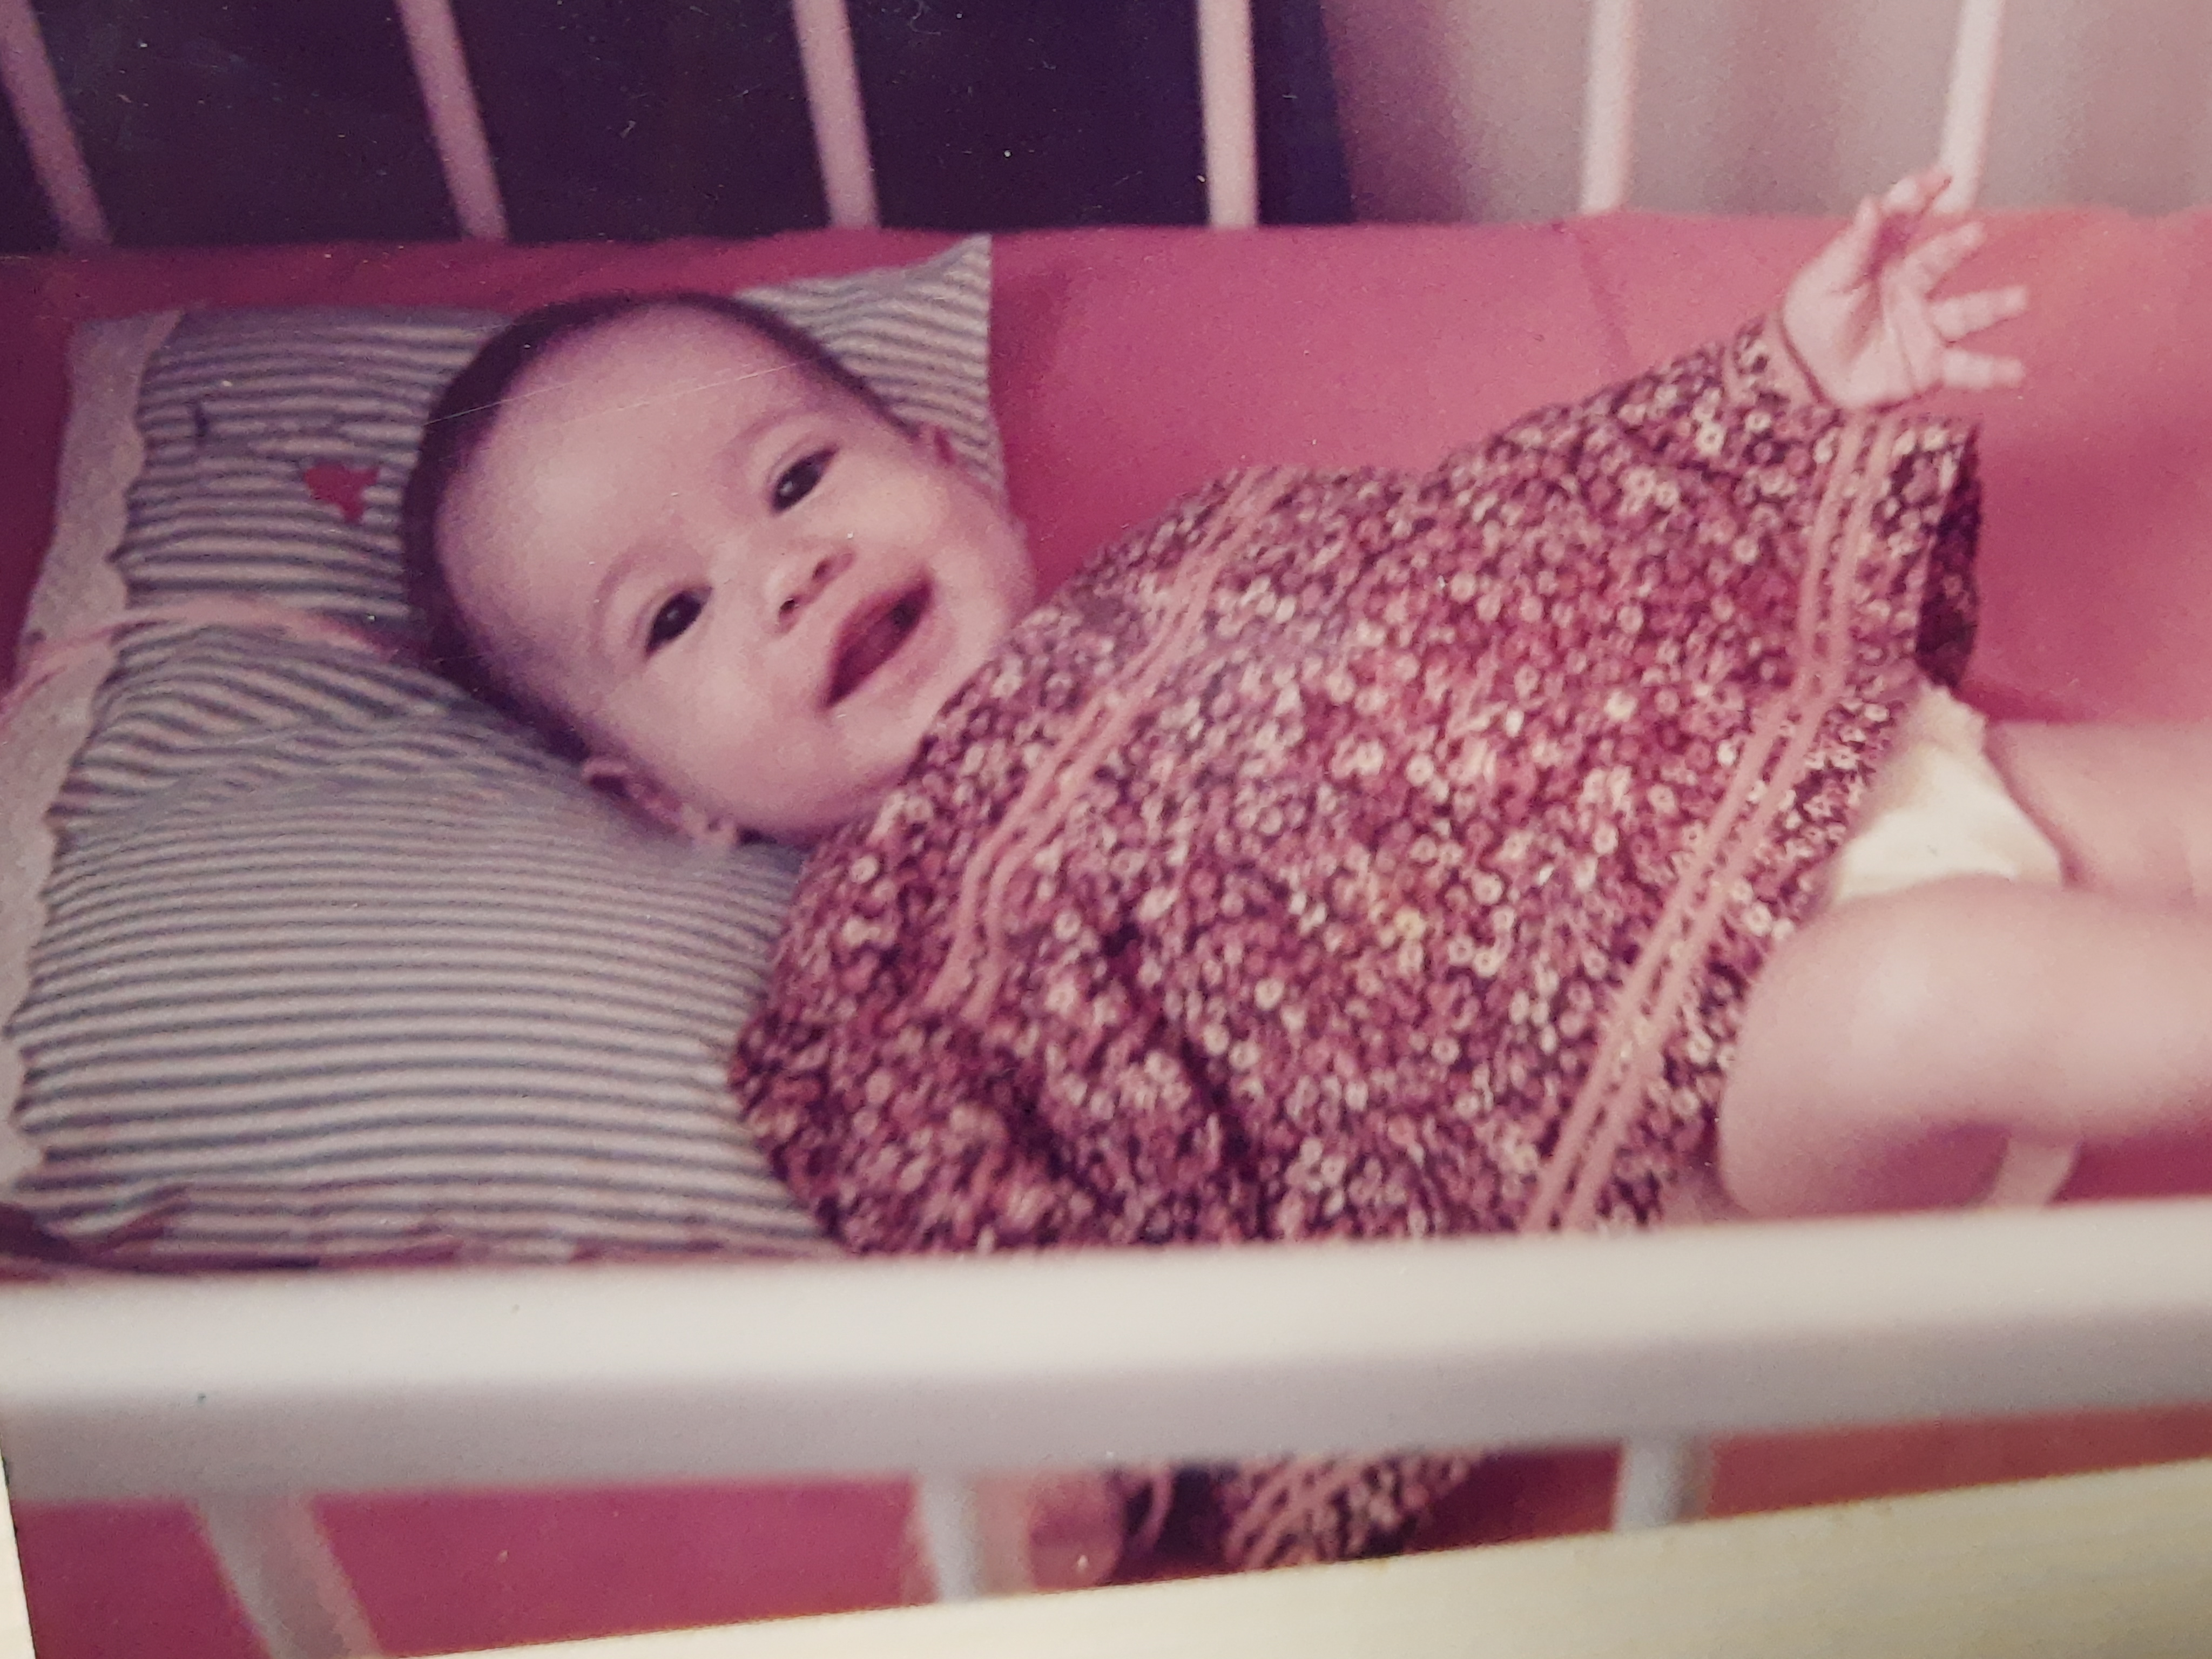
\includegraphics{img/reta_baby_1.jpg}
\caption{Pequena Renata}
\end{figure}

\begin{figure}
\centering
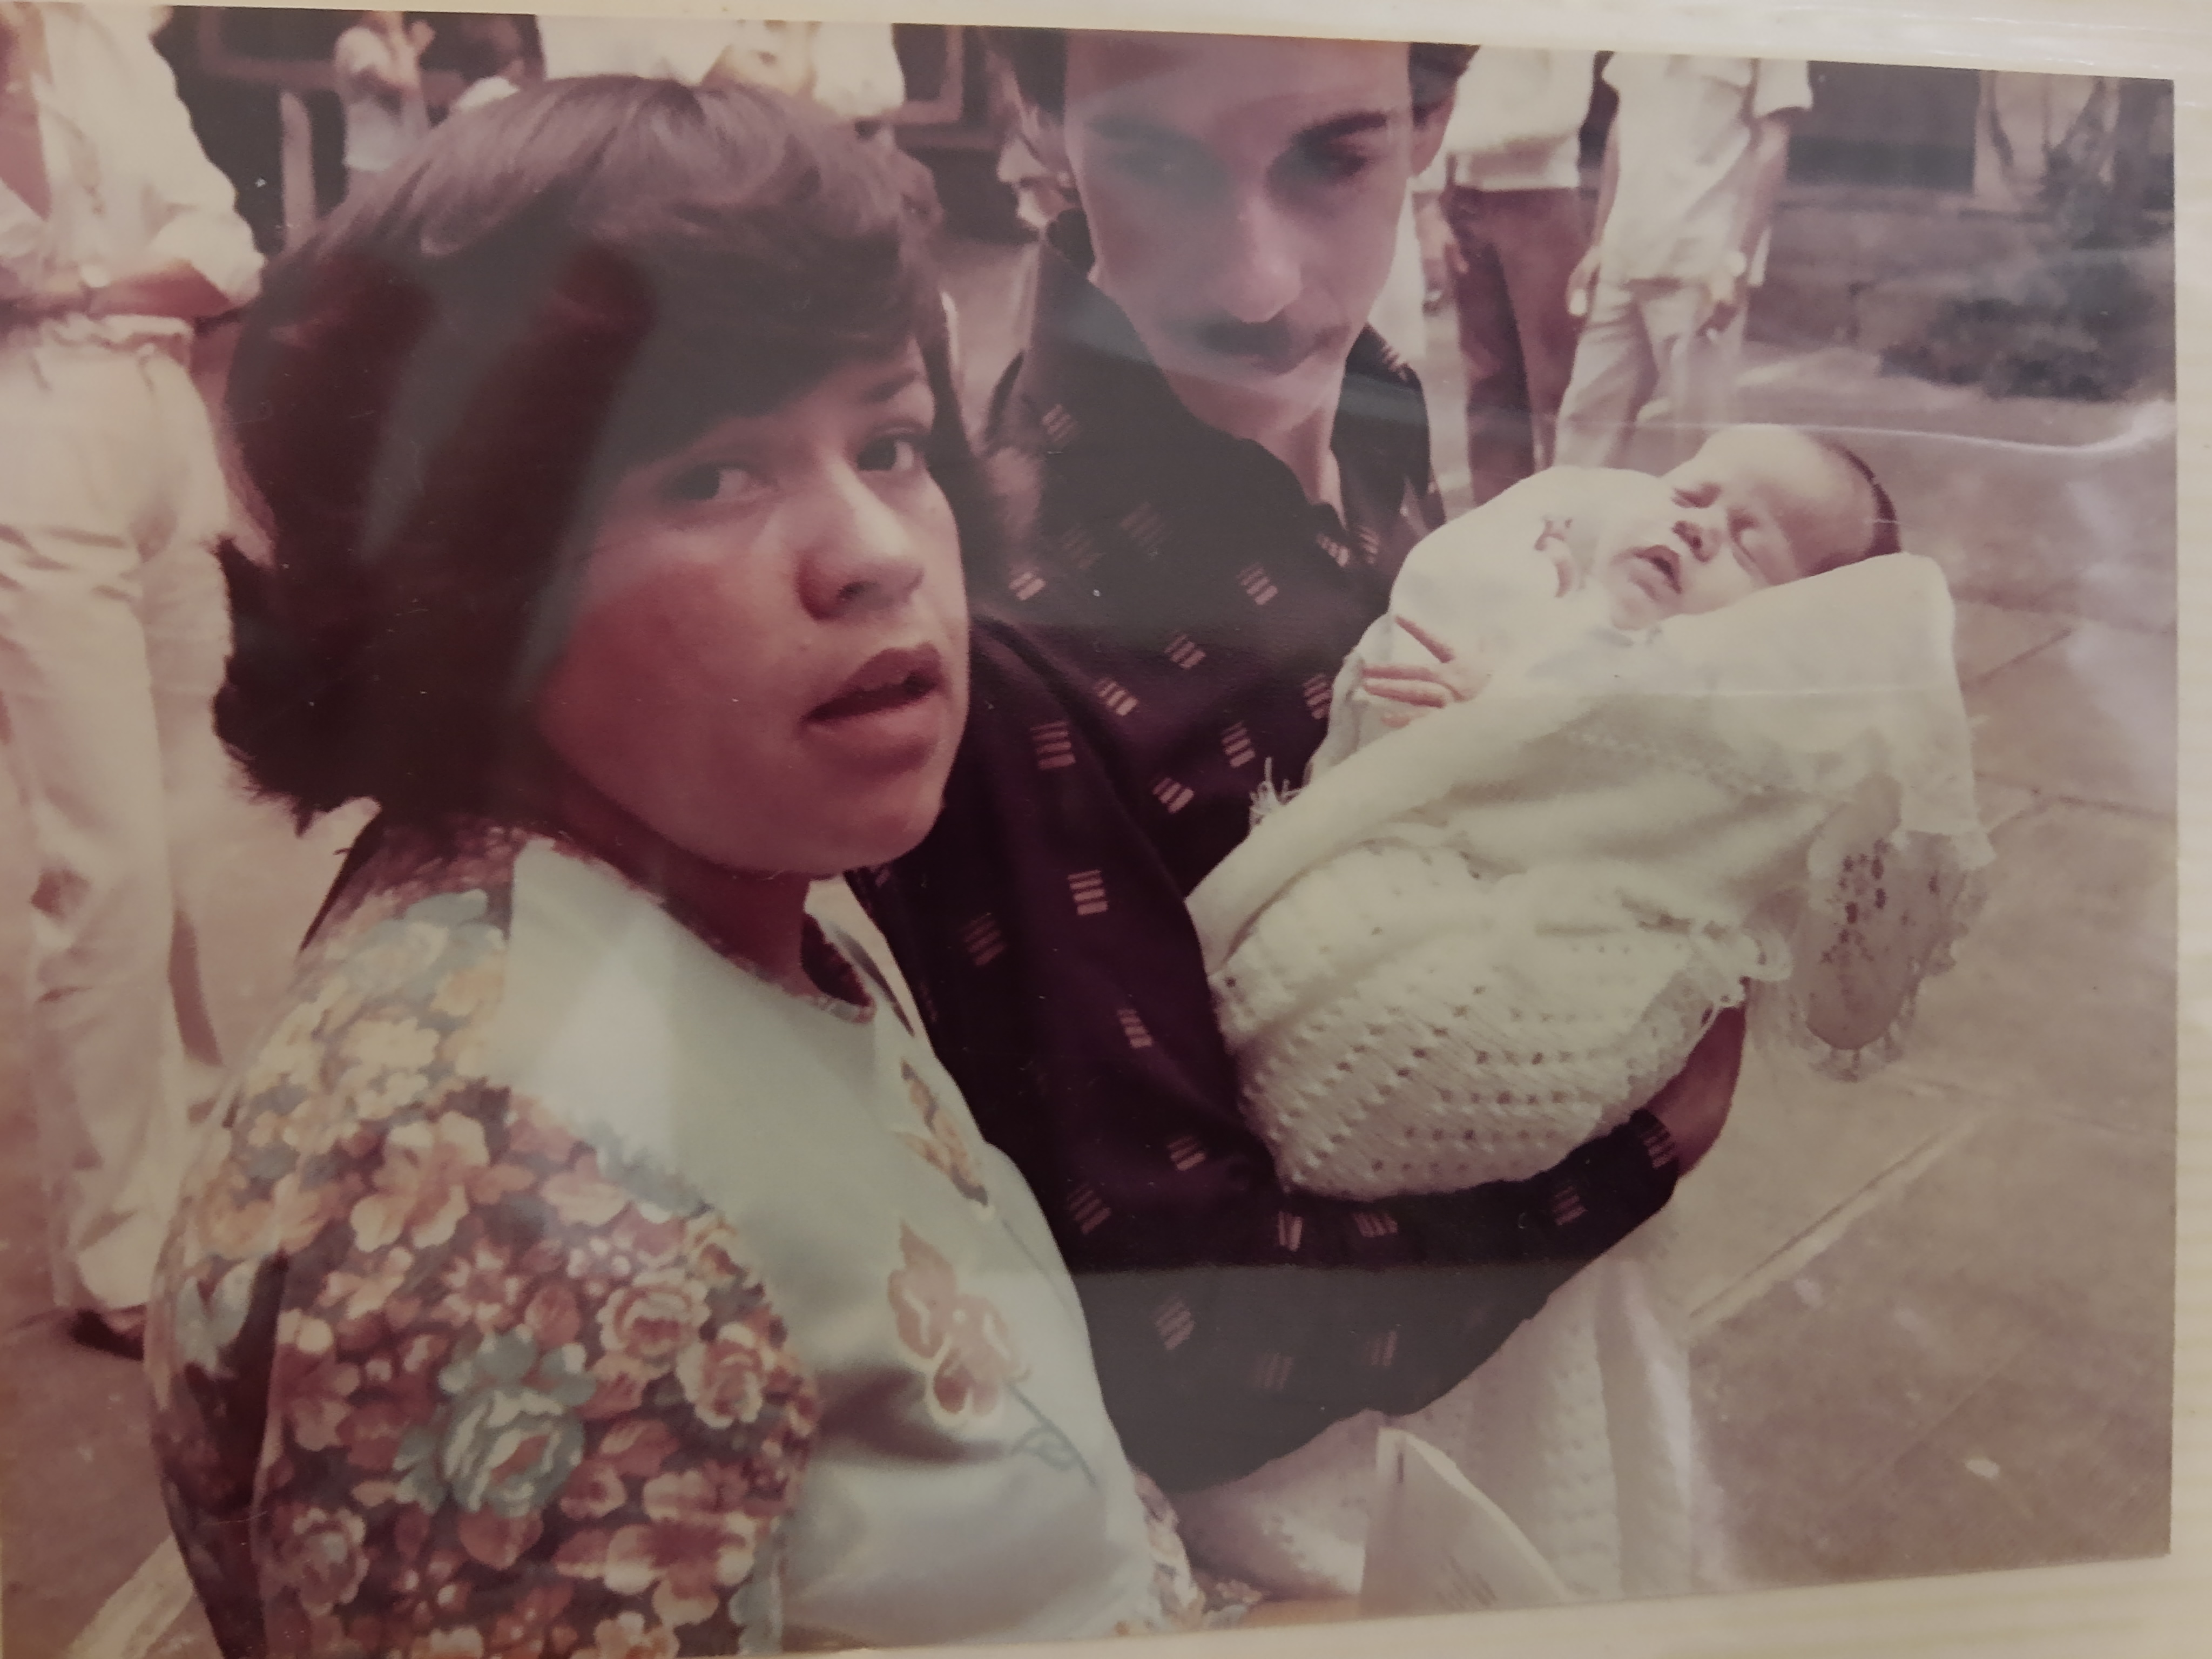
\includegraphics{img/pais.jpg}
\caption{Lúcia, Odimar e Renata}
\end{figure}

Meus pais trabalhavam em tempo integral e eu ficava sob cuidados da
minha avó \emph{Gecy de Oliveira Magalhães} (@ref(fig:gecy) e de
funcionárias domésticas. Minha avó foi uma das pessoas mais importantes
na construção do meu caráter, da minha personalidade e da minha
essência. Infelizmente ela não se encontra mais neste plano terreno, mas
com certeza preenche um pedaço enorme do meu coração. Naquela época a
educação era um efetivo caminho para o acesso a oportunidades. Meus pais
se esforaçaram para pagar mensalidades de escola particular, cursos
complementares de língua, datilografia, artes. Estudei no Colégio Santa
Doroteia\footnote{Escola confessional católica tradicional de Belo
  Horizonte \href{https://santadoroteia.com.br}{Site}}. Naquele
contexto, era a melhor educação formal que os pais poderiam proporcionar
aos filhos. Ainda considerando a educação como instrumento de
transformação, meus pais viabilizaram que eu me tornasse proficiente em
língua inglesa e em datilografia\footnote{Materializando as quatro
  décadas da minha existência 🥰.}.

\begin{figure}
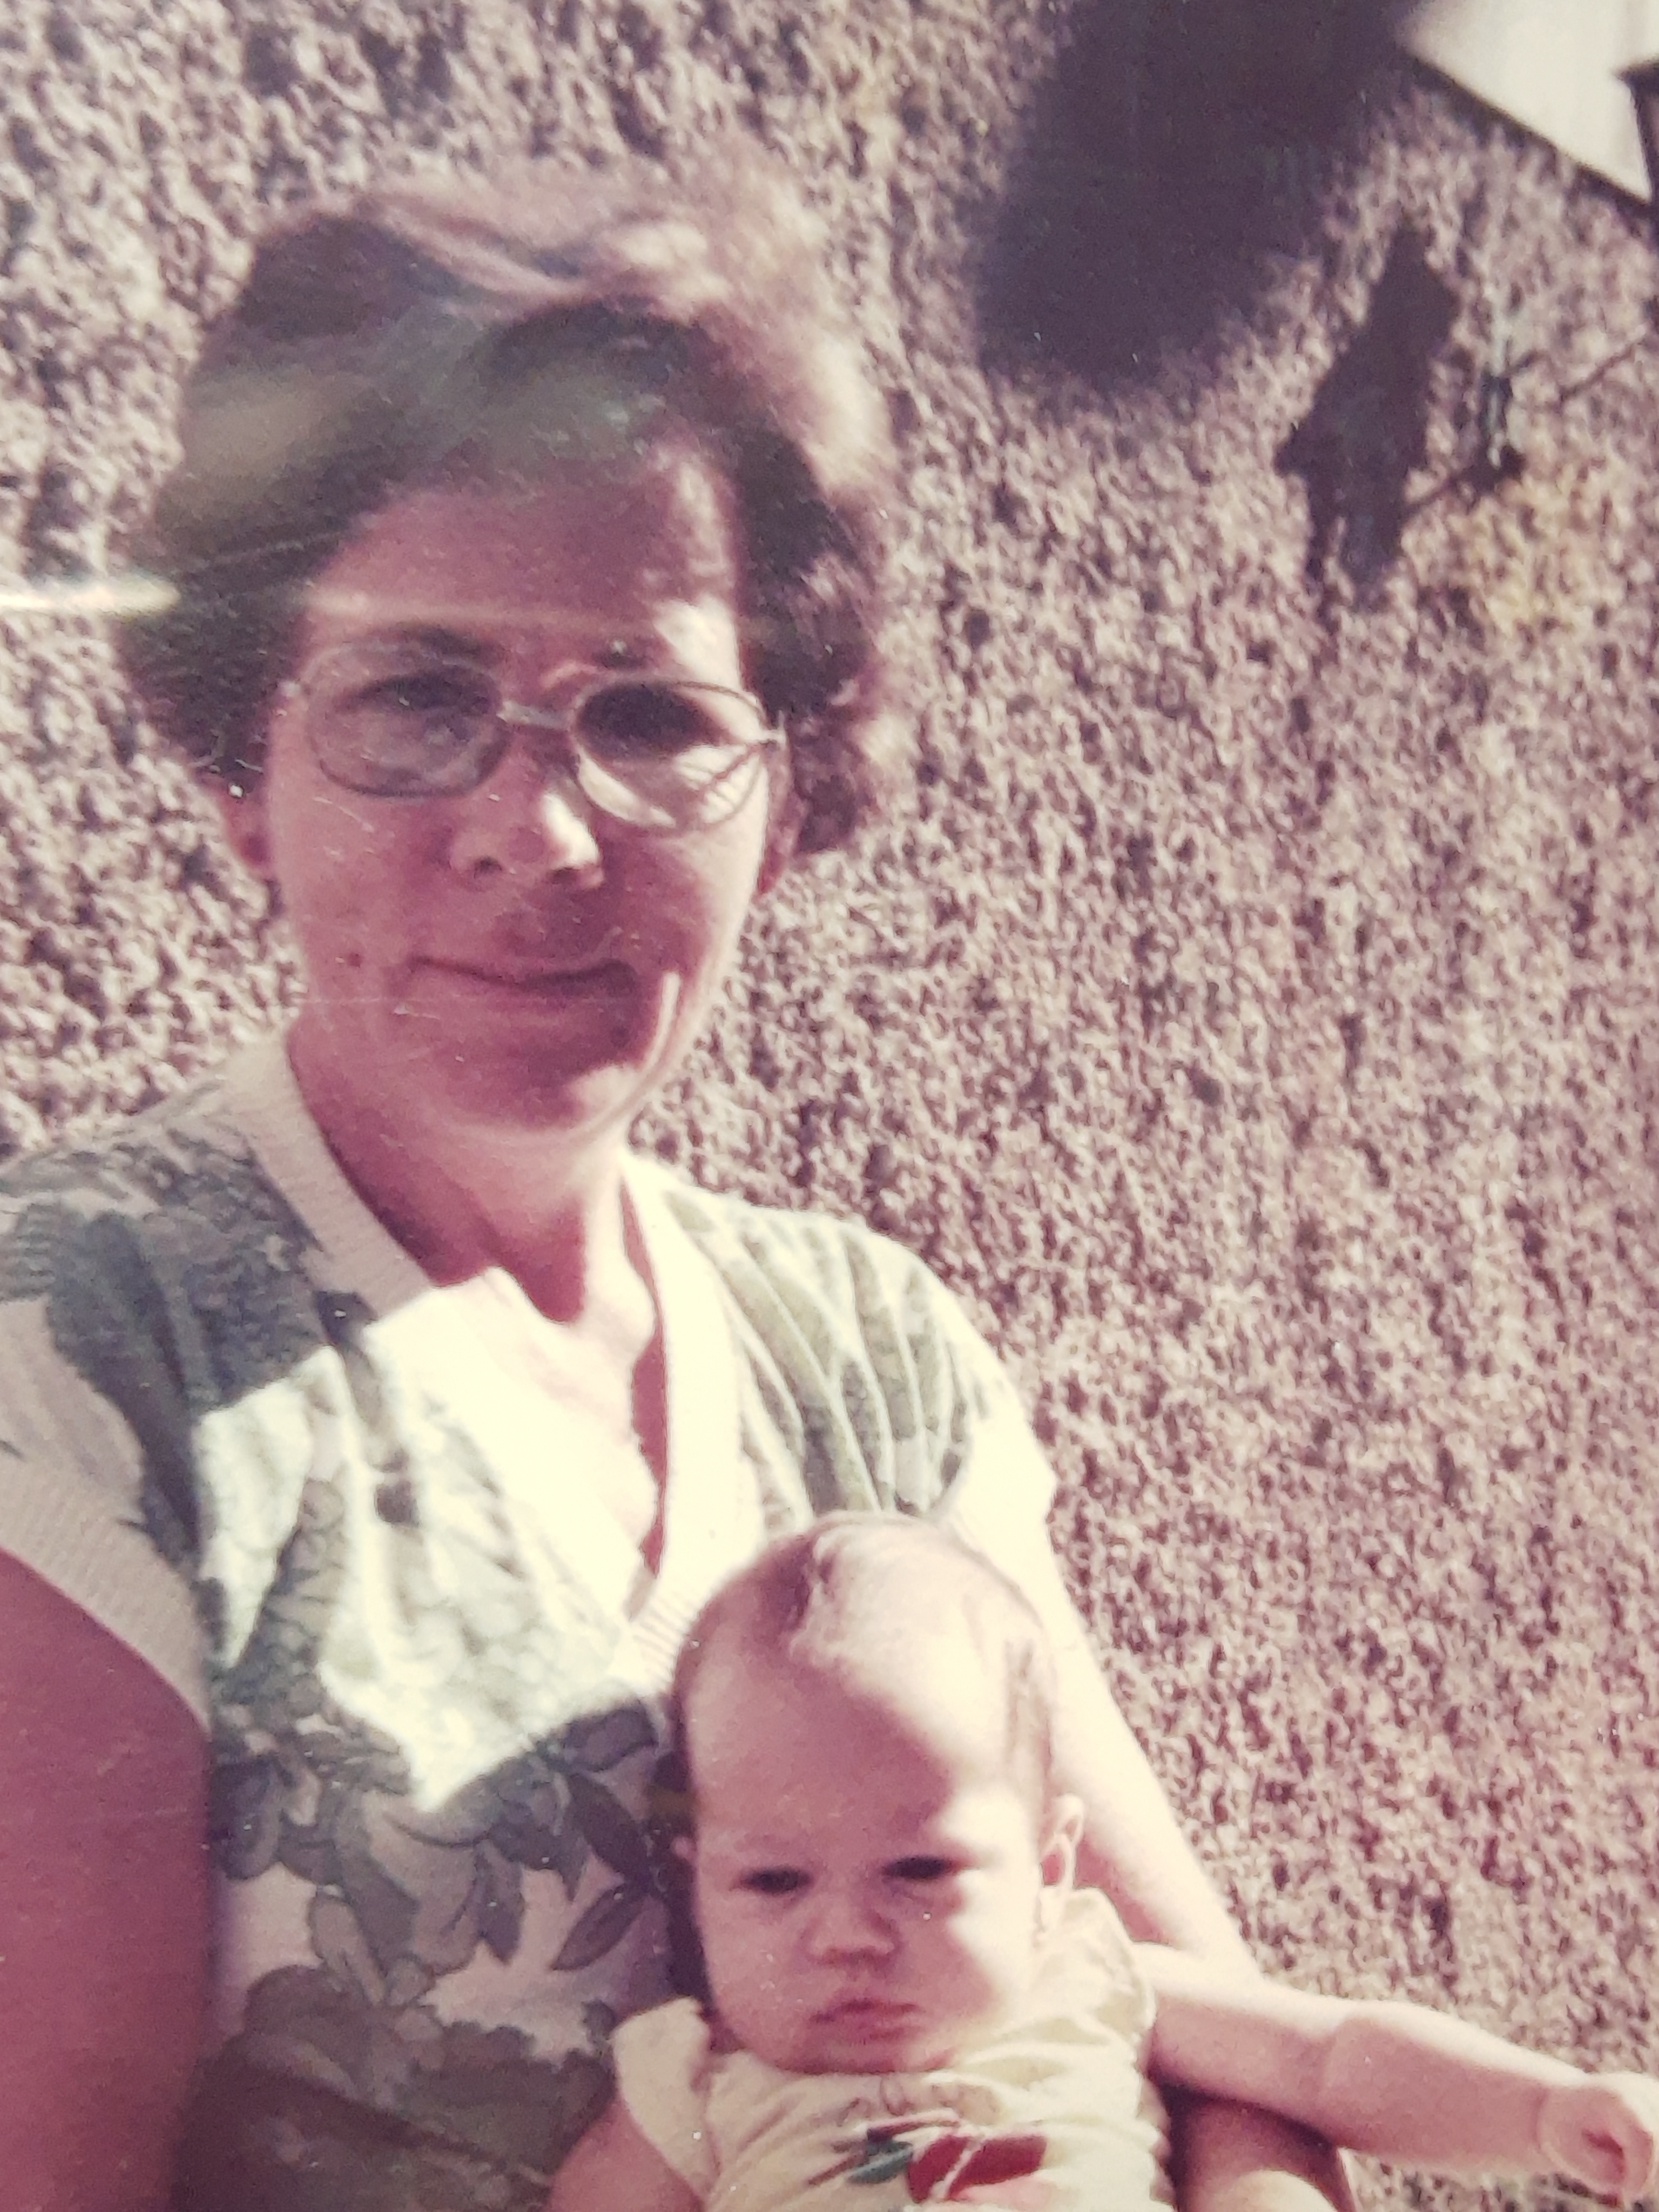
\includegraphics[width=1\linewidth]{img/gecy} \caption{Gecy e Renata}\label{fig:gecy}
\end{figure}

Sempre foi uma estudante dedicada e preocupada com o desempenho
acadêmico, sem, no entanto, considerar que o êxito acadêmico no sistema
de ensino tradicional revelaria algo sobre mim ou me colocaria em
posição diferente dos meus coleges e amiges. Entretanto, até o início da
adolescência, sempre fui bastante introspectiva e tímida.

Dos 4 aos 16 anos nadei, nadei, nadei\ldots. 🏊🏊🏊🏊 e estudei 📚, sendo a
repetição das palavras um \emph{proxy} da intensidade dessas atividades
na minha rotina. Ao longo da adolescência fui descobrindo novas maneiras
de me relacionar com as pessoas, o que foi muito positivo também nos
caminhos que construí para a vida profissional.

Aos 16 anos me aventurei na primeira experiência internacional. Morei
como estudante de \emph{High School} por 6 meses nos Estados Unidos, no
estado \textbf{Idaho}\footnote{Não se preocupe se nunca ouviu falar. É
  realmente um lugar conhecido apenas por suas batatas maravilhosas 🥔!}.
Foi uma experiência maravilhosa. Em meados da década 1990, a internet
era um advento tecnológico disponível apenas em centros acadêmicos e as
ligações telefônicas tinham preços proibitivos! Nosso principal meio de
comunicação era o correio convencional e a troca de cartas.

Quando retornei desse período de intercâmbio, \ldots{}\footnote{Minha
  trajetória como docente é apresentada nos próximos episódios.}

\hypertarget{universalidade-da-docuxeancia-como-profissuxe3o}{%
\chapter{Universalidade da docência como
profissão}\label{universalidade-da-docuxeancia-como-profissuxe3o}}

O mundo do trabalho sempre esteve presente na minha vida. Seja por conta
das atividades profissionais que meus pais exerciam ou seja pela minha
vontade, a partir da adolescência, de ser independente. O trabalho se
mostrou como parte natural da minha vida muito cedo, mas não por
necessidade. A condição financeira da minha família foi determinante no
meu \textbf{acesso} à educação e, caso fosse meu desejo, poderia deixar
para ingressar no mundo do trabalho mais tarde. Entretanto, apesar da
minha insegurança em relação às minhas competências, a vontade

E claro, a docência fez parte desse mundo desde o início. Minha primeira
atividade profissional foi como professora de inglês.

Quando retornei de um intercâmbio nos Estados Unidos aos 16 anos,
comecei a lecionar.

Escolher a profissão é sempre um desafio, especialmente quando somos
muito jovens e associamos a perspectiva do trabalho às disciplinas que
cursamos ao longo da educação básica. De fato, eu já tinha uma profissão
quando precisei preencher o formulário de inscrição para o vestibular
com minhas opções de curso universitário.

Durante muitos anos eu fui apaixonada por biologia, mais especificamente
por zoologia, mas não poderia dissecar um animal em laboratório.
Entretanto, no ensino médio, fiquei apaixonada por química e física.
Cheguei a pensar (nem acredito nisso hoje) em cursar física básica no
ensino superior. Entretanto, e também devido à influência das escolhas
profissionais da minha mãe, considerei as engenharias como o caminho
profissional mais alinhado com minha vocação. Hoje acredito que todos
temos vocação para quaisquer áreas de conhecimento. Basta que estejamos
motivados.

Dentre as engenharias, a minha primeira opção seria cursar engenharia
química; bem intuitivo. Entretanto, quando ingressei na universidade, em
1997, havia uma recessão econômica que limitava bastante as
oportunidades de trabalho para engenheiros. Assim, a minha linha de
pensamento foi escolher o curso universitário conforme empregabilidade
ou possibilidade de exercer a profissão informalmente. Assim, dentre as
diversas opções em engenharia, a engenharia civil pareceu mais versátil
para que eu pudesse, eventualmente, ter uma fonte de renda, mesmo que
informal.

E foi assim. Fiz vestibular para engenharia civil e fui aprovada na
FUMEC, PUCMinas e UFMG. Felizmente, ao ser aprovada nas três
isntituições, pude escolher e comecei, em fevereiro de 1997, o curso de
engenharia civil na UFMG.

Instituto de ciências exatas e laboratórios de topografia foram minha
casa durante dois anos, que consolidam o ``ciclo básico'' das
engenharias. Durante esse período eu não consegui explorar a engenharia
como profissão. Eram disciplinas nada aplicadas e eu seguia exercendo
minha atividade profissional como professora de inglês. Em 1997 consegui
uma colocação em uma escola de línguas e, pela primeira vez, tive acesso
a um curso de qualificação para exercer o ensino de língua estrangeira.
Foi um diferencial naquele momento da minha vida, pois percebi que,
apesar de adorar lecionar, havia também muita técnica e processos que
potencialmente melhorariam minhas aulas.

Segui lecionando nessa escola por um ano. Após esse período, optei por
ministrar aulas particulares e em grupos e consegui manter essa
atividade como minha profissão e fonte de renda até o meio do curso de
graduação. No sexto período, resolvi investir na minha formação em
engenharia e fazer um estágio em uma construtora, para explorar os
caminhos que a engenharia civil possibilitava. Fiz estágio em um setor
de orçamento de obras e não consegui cumprir meu contrato de seis meses.
Pedi desligamento no quinto mês, pois não conseguia me dedicar a fazer
as mesmas atividades diariamente durante o mês.

Como meu dia tem apenas 24 horas (às vezes ainda esqueço disso),
precisei reduzir minha carga de aulas de inglês e, no sétimo período,
consegui uma vaga como bolsista de iniciação científica. O projeto era
intitulado ``\textbf{Mobilidade} Residencial e Sistema de Transporte na
Região Metropolitana de Belo Horizonte'' e foi desenvolvido no
Departamento de Engenharia de Transportes e Geotecnia sob orientação do
professor \emph{David José Ahouagi Vaz de Magalhães}.

Ao final do curso, não tive dúvidas de que precisaria aprofundar meus
conhecimentos após ter escolhido a área de engenharia de transportes
para atuação. Na graduação, as disciplinas dessa área de conhecimento
são abrangentes e têm como objetivo apresentar os grandes tópicos que
compõe a engenharia de transportes. Infelizmente, em Belo Horizonte, não
havia a possibilidade de realizar um mestrado nessa área. Assim,
pesquisei alguns programas, coletei algumas informações sobre como
montar um pre-projeto de pesquisa e fiz a inscrição nos programas da
USP-São Carlos, da UFRJ e do IME. A inscrição na UFRJ e no IME foi
presencial e, naquele momento, me decidi pelo IME. Não por conta
essencialmente da qualidade do curso, mas devido à \textbf{localização}
do IME em relação ao Campus da UFRJ na ilha do função. A
\textbf{localização} já se manifestava como instrumento de
\textbf{decisão} na minha vida.

Fui aprovada nos três programas e decidi ir para o Rio de Janeiro, me
matriculando no IME. O principal fator para escolha do Rio e não de São
Carlos estava relacionado ao coração, e a \textbf{distância} entre Belo
Horizonte e as respectivas cidades foi decisiva.

Cresci acreditando que as pessoas conseguem conquistas bens materiais e
status por meio de esforço e mérito individual. Acreditava que a
possibilidade de gerar valor para as empresas era o que diferenciava um
bom engenheiro de um mau profissional. Assim, evitando olhar para o
público, direcionei o meu projeto de mestrado para o transporte de
cargas, entendendo, naquele momento, que estaria isenta de decisões
públicas interferindo no meu projeto acadêmico e na minha atividade
profissional.

Assuntos do coração têm um capítulo especial neste memorial, pois
tiveram um papel importante na maior parte das escolhas profissionais e
acadêmicas que fiz.

2003 foi um ano meio de mudanças. Mudanças de emprego, de casa e de
objetivos. Após cumprir os créditos básicos no IME, resolvi trancar o
curso e voltar para Belo Horizonte. Como não consegui ficar sem
trabalhar, busquei estágio na empresa-referência em consultoria de
transportes em BH naquela época: o grupo Tectran. Bati à porta do
escritório da Tectran, com meu singelo currículo embaixo do braço e
perguntei se tinham alguma vaga para mim. Acharam estranho essa
abordagem, mas coloquei-me à disposição inclusive para estagiar como
mestranda na empresa e me fizeram a proposta de trabalhar como
estagiária recebendo remuneração equivalente àquela da bolsa de mestrado
da época. Foi maravilhoso. A equipe era acolhedora e, como o grupo ainda
era pequeno, tive a oportunidade de colaborar com projetos em diferentes
áreas e de, efetivamente, aprender a trabalhar. Penso que essa tenha
sido a minha primeira experiência profissional como engenheira e adorei!
Adorei não fazer a mesma coisa todos os dias, adorei eventualmente
estudar para propor algum caminho metodológico para os projetos e de
efetivamente concluir etapas ao longo da vida profissional.

Eu nunca me senti confortável em não experimentar a concepcão, o
desenvolvimento e o fechamento das minhas atividades. Não ver o
resultado da minha contribuição, seja como professora ou como
engenheira, me desmotivava e não

E que a minha aventura como professora de inglês aos 16 anos foi
bastante audaciosa e exitosa. Comecei a lecionar para uma amiga e uma
tia que encararam a experiência. Sofia falou que o êxito como professora
era, possivelmente, resultado da inexperiência e da vontade de fazer
diferente. Sem preconceitos e sem expectativas, construí intuitivamente

Ao longo da elaboração deste memorial, comentei com minha filha Sofia
(na seção de assuntos do coração vocês conhecerão como ela veio fazer
parte da minha essência) que eu sempre me motivei mais com atividades
que apresentavam início, meio e fim.

Em 2003, em meio às atividades de consultoria, consegui uma colocação,
aos 24 anos, para atuar como professora na Faculdade Novos Horizonte.
Apostaram em mim, mesmo

Lecionei Logística

Entrei na vale em setembro de 2003 e etapa mais difícil do processo
seletivo foi pedir demissão da minha posição de estagiária na Tectran.
Tinha aprendido tanto e nutria afeto pelas pessoas e pelo acolhimento
recebido. Mas a vida segue e me desligar daquela posição não era fechar
portas e sim buscar novas experiências. Quando ao processo seletivo,
foram inúmeras etapas e, mais uma vez, contei com minha formação ao
longo da vida e entrei no processo de maneira despretenciosa, por
indicação do amigo \emph{Maurício Aguiar}.

Foi curioso que, durante o processo seletivo, passei por dois gerentes
gerais na entrevista final. O primeiro a me entrevistar identificou
minha inaptidão a rotinas e, portanto, a trabalhar na operação. O que
não é rotina na operação ferroviária, é problema! O primeiro gerente a
me entrevistar me encaminhou para o segundo e o resultado foi que fui a
única ``Engenheira Ferroviária'' que não estava lotada na Diretoria de
Operações. Fui alocada em uma área de estudos operacionais sob a
Diretoria de Planejamento. Essa decisão dos gestores foi muito assertiva
e alinhada com o meu potencial de contribuição para a empresa.

Assumimos na Vale, eu e meus colegas e amigos Engenheiros Ferroviários,
no dia 15 de setembro de 2003. Entramos na primeira edição do programa
de trainee ``Engenheiro Ferroviário,'' cujo objetivo era capacitar
jovens talentos para atuar no mercado ferroviário. Por anos não houve
investimento em mão de obra para operação e gestão de ferrovias. Assim,
fez necessário que as operadoras investissem em qualificação, como ainda
é realidade nesse setor.

Foram três meses de aulas e muita aprendizagem. Também, de viagens,
companheirismo e construção de novas amizades. Essa capacitação
aconteceu em imersão no saudoso Othon Palace Hotel de Belo Horizonte e
posteriormente viajamos visitando as diferentes instalações ferroviárias
da Vale nas ferrovias Estrada de Ferro Vitória a Minas, Estrada de Ferro
Carajás e Ferrovia Centro Atlântica. Felizmente, durante o treinamento,
fiquei em casa (assuntos do coração são fortes!) e frequentei as aulas
diárias.

Aprendemos muito e ao final, fui alocada para desenvolver projetos
internos de melhoria, trabalhando com simulação de trens\ldots.

Eu respirava engenharia econômica e até restaurantes foram apelido pela
equipe como VPL, por apresentarem um ótimo custo-benefício. Aprendi que
a qualidade do meu trabalho é diretamente proporcional ao tempo que
tenho para fazê-lo. Tive que aprender a controlar a vontade de fazer
melhor, pois os prazos não eram flexíveis e a entrega tinha que
acontecer. Aprendi também que uma empresa como a Vale, apesar de
permeada de processos decisórios exclusivamente fundamentados em uma
disputa de poder de mercado e política, era orientada à remuneração de
capital. Que princípios éticos, que a qualidade técnica da engenharia e
até mesmo as situações de risco podem ser descartados se remunerarmos o
acionista. Eu precisava transformar o resultado de estudos de melhoria
operacional em resultado financeiro. ``Dá VPL?'' Era a pergunta do
diretor na decisão de investimento.

Alguns meses depois, houve, durante uma das muitas reestruturações
gerenciais, a demanda de ume profissional na área de planejamento
ferroviário no longo e médio prazos. Essa área era a interface entre as
funções comerciais e operacionais da ferrovia e trabalhávamos
organizando os fluxos a serem realizados nos horizontes mensal e anual.
Foi maravilhoso entender um pouco mais sobre o sistema ferroviário como
serviço e me tornar uma das pessoas responsáveis pelo dimensionamento de
vagões, locomotivas e o arranjo dos trens com todas as restrições que a
ferrovia . Mas o encatamento

Fui responsável pela coordenação de dados obtidos a partir de diferentes
ERPs (Enterprise Resource Planning) que eram os sistemas de gestão
diferentes para cada ferrovia. Recebia ainda dados das áreas de
manutenção de material rodante e via permanente. Consolidando e
coordenando as informações, gerávamos um instrumento denominado Book PPC
(planejamento, programação e controle) que era um conjunto de planilhas
com indicadores de desempenho ferroviários. Aquele documento era
encaminhado para toda a Diretoria de Logística visando acompanhamento de
metas e resultados, nas diferentes dimensões que eram possíveis

Hoje faço dessa experiência a base para construção do conhecimento em
ciência de dados e para que eu consiga apresentar esse conteúdo de forma
aplicada para os alunos.

Durante meu período na Vale, de setembro de 2003 a maio de 2005, não
consegui coordenar minhas atividades como docente e, portanto, solicitei
suspensão do meu contrato na Faculdade Novos Horizontes e fiquei até
2005 vinculada à instituição, mas sem lecionar. Mais uma vez sou grata
pela confiança e pela oportunidade de obter experiência na docência no
ensino superior.

Em 2005, após pedir desligamento da Vale, lecionei em faculdades
particulares em cursos de administração e como professora substituta de
volta ao Departamento de Engenharia de Transportes e Geotecnia da UFMG.
As faculdades particulares - FUNCESI - Fundação Uni\ldots. e Novos
Horizonte foram oportunidades únicas pois conseguir colocações
profissionais sem experiência praticamente inviabiliza a construção de
experiências. É o ciclo perverso do início da carreira de qualquer
jovem. Nessas universidade lecionei disciplinas relacionadas à gestão
das operações e à aplicação de métodos quantitativos, como administração
da produção, da qualidade e logística. Essas disciplinas estavam
relacionadas com minha formação básica na engenharia civil e minha
especialização no mestrado.

Quando fui professora substituta na UFMG, enfrentei um desafio
profissional que tinha um peso emocional importante. O professor
\emph{Baeta} precisou se aposentar por idade e eu assumiria seu lugar.
Ele, como sempre, foi muito solícito ao fazer um processo suave de
transição das disciplinas. Entretanto, eu me sentia mal por assumir seu
lugar, sendo que ele ainda gostaria de exercer a docência. Ainda,
discordava de algumas práticas em sala de aula adotadas por ele quando
estudante e queria fazer diferente.

Escolha pela docência Lecionar no contexto dos centros educacionais
privados, hoje em protagonismo no cenário atual. Casamento Concurso para
o CEFET

\hypertarget{escolhas-profissionais-e-caminhos-acaduxeamicos}{%
\chapter{Escolhas profissionais e caminhos
acadêmicos}\label{escolhas-profissionais-e-caminhos-acaduxeamicos}}

O mundo do trabalho sempre esteve presente na minha vida. Seja por conta
das atividades profissionais que meus pais exerciam ou seja pela minha
vontade, a partir da adolescência, de ser independente. O trabalho se
mostrou como parte natural da minha vida muito cedo, mas não por
necessidade. A condição financeira da minha família foi determinante no
meu \textbf{acesso} à educação e, caso fosse meu desejo, poderia deixar
para ingressar no mundo do trabalho mais tarde. Entretanto, apesar da
minha insegurança em relação às minhas competências, a vontade

E claro, a docência fez parte desse mundo desde o início. Minha primeira
atividade profissional foi como professora de inglês.

Quando retornei de um intercâmbio nos Estados Unidos aos 16 anos,
comecei a lecionar.

\hypertarget{graduauxe7uxe3o}{%
\section{Graduação}\label{graduauxe7uxe3o}}

Escolher a profissão é sempre um desafio, especialmente quando somos
muito jovens e associamos a perspectiva do trabalho às disciplinas que
cursamos ao longo da educação básica. De fato, eu já tinha uma profissão
quando precisei preencher o formulário de inscrição para o vestibular
com minhas opções de curso universitário.

Durante muitos anos eu fui apaixonada por biologia, mais especificamente
por zoologia, mas não poderia dissecar um animal em laboratório.
Entretanto, no ensino médio, fiquei apaixonada por química e física.
Cheguei a pensar (nem acredito nisso hoje) em cursar física básica no
ensino superior. Entretanto, e também devido à influência das escolhas
profissionais da minha mãe, considerei as engenharias como o caminho
profissional mais alinhado com minha vocação. Hoje acredito que todos
temos vocação para quaisquer áreas de conhecimento. Basta que estejamos
motivados.

Dentre as engenharias, a minha primeira opção seria cursar engenharia
química; bem intuitivo. Entretanto, quando ingressei na universidade, em
1997, havia uma recessão econômica que limitava bastante as
oportunidades de trabalho para engenheiros. Assim, a minha linha de
pensamento foi escolher o curso universitário conforme empregabilidade
ou possibilidade de exercer a profissão informalmente. Assim, dentre as
diversas opções em engenharia, a engenharia civil pareceu mais versátil
para que eu pudesse, eventualmente, ter uma fonte de renda, mesmo que
informal.

E foi assim. Fiz vestibular para engenharia civil e fui aprovada na
FUMEC, PUCMinas e UFMG. Felizmente, ao ser aprovada nas três
isntituições, pude escolher e comecei, em fevereiro de 1997, o curso de
engenharia civil na UFMG.

Eu aproveitei bastante a minha vida acadêmica no ensino superior.
Explorei algumas das oportunidades ofertadas pela universidade
\textbf{pública}, me envolvendo em diferentes atividades. Participei de
diferentes instâncias da representação estudantil: (i) compûs diferentes
gestões do Grêmio Estudantil da Engenharia Civil; (ii) envolvi-me em
projetos do Diretório Acadêmico das engenharias; (iii) representei o
corpo discente em reuniões departamentais e em outros colegiados; (iv)
aprendi a me posicionar de maneira adversa ao senso comum nos órgãos
colegiados para levar a perspectiva estudantil para a discussão; (v)
aprendi como funcionam os departamentos acadêmicos das universidades em
seus bastidores. E claro, foi no contexto universitário que meu coração
se tornou mais vermelhinho e feliz (assunto para a seção ``assuntos do
coração'').

Além de cursar Engenharia Civil como apresentei no capítulo referente às
escolhas profissionais, no oitavo período desse curso, já colaborando
formalmente com o projeto de iniciação científica, resolvi experimentar
outro curso de graduação. Intuitivamente pensei em letras, mas entendi
que não haveria contribuição direta para a minha formação profissional.
Resolvi estudar comércio exterior e fiz um vestibular para uma faculdade
particular chamada UNA. Fui aprovada e cursei no período noturno um
semestre de comex. Não me adaptei à instituição, ao curso e ao contexto
e acabei cursando apenas o primeiro semestre.

No dia 08 de Janeiro de 2002 colei grau como Engenheira Civil da UFMG
(@ref(fig:forma)).\footnote{Deixo para vocês a brincadeira de ``onde
  está Renata'' na foto! 🤪}

\begin{figure}
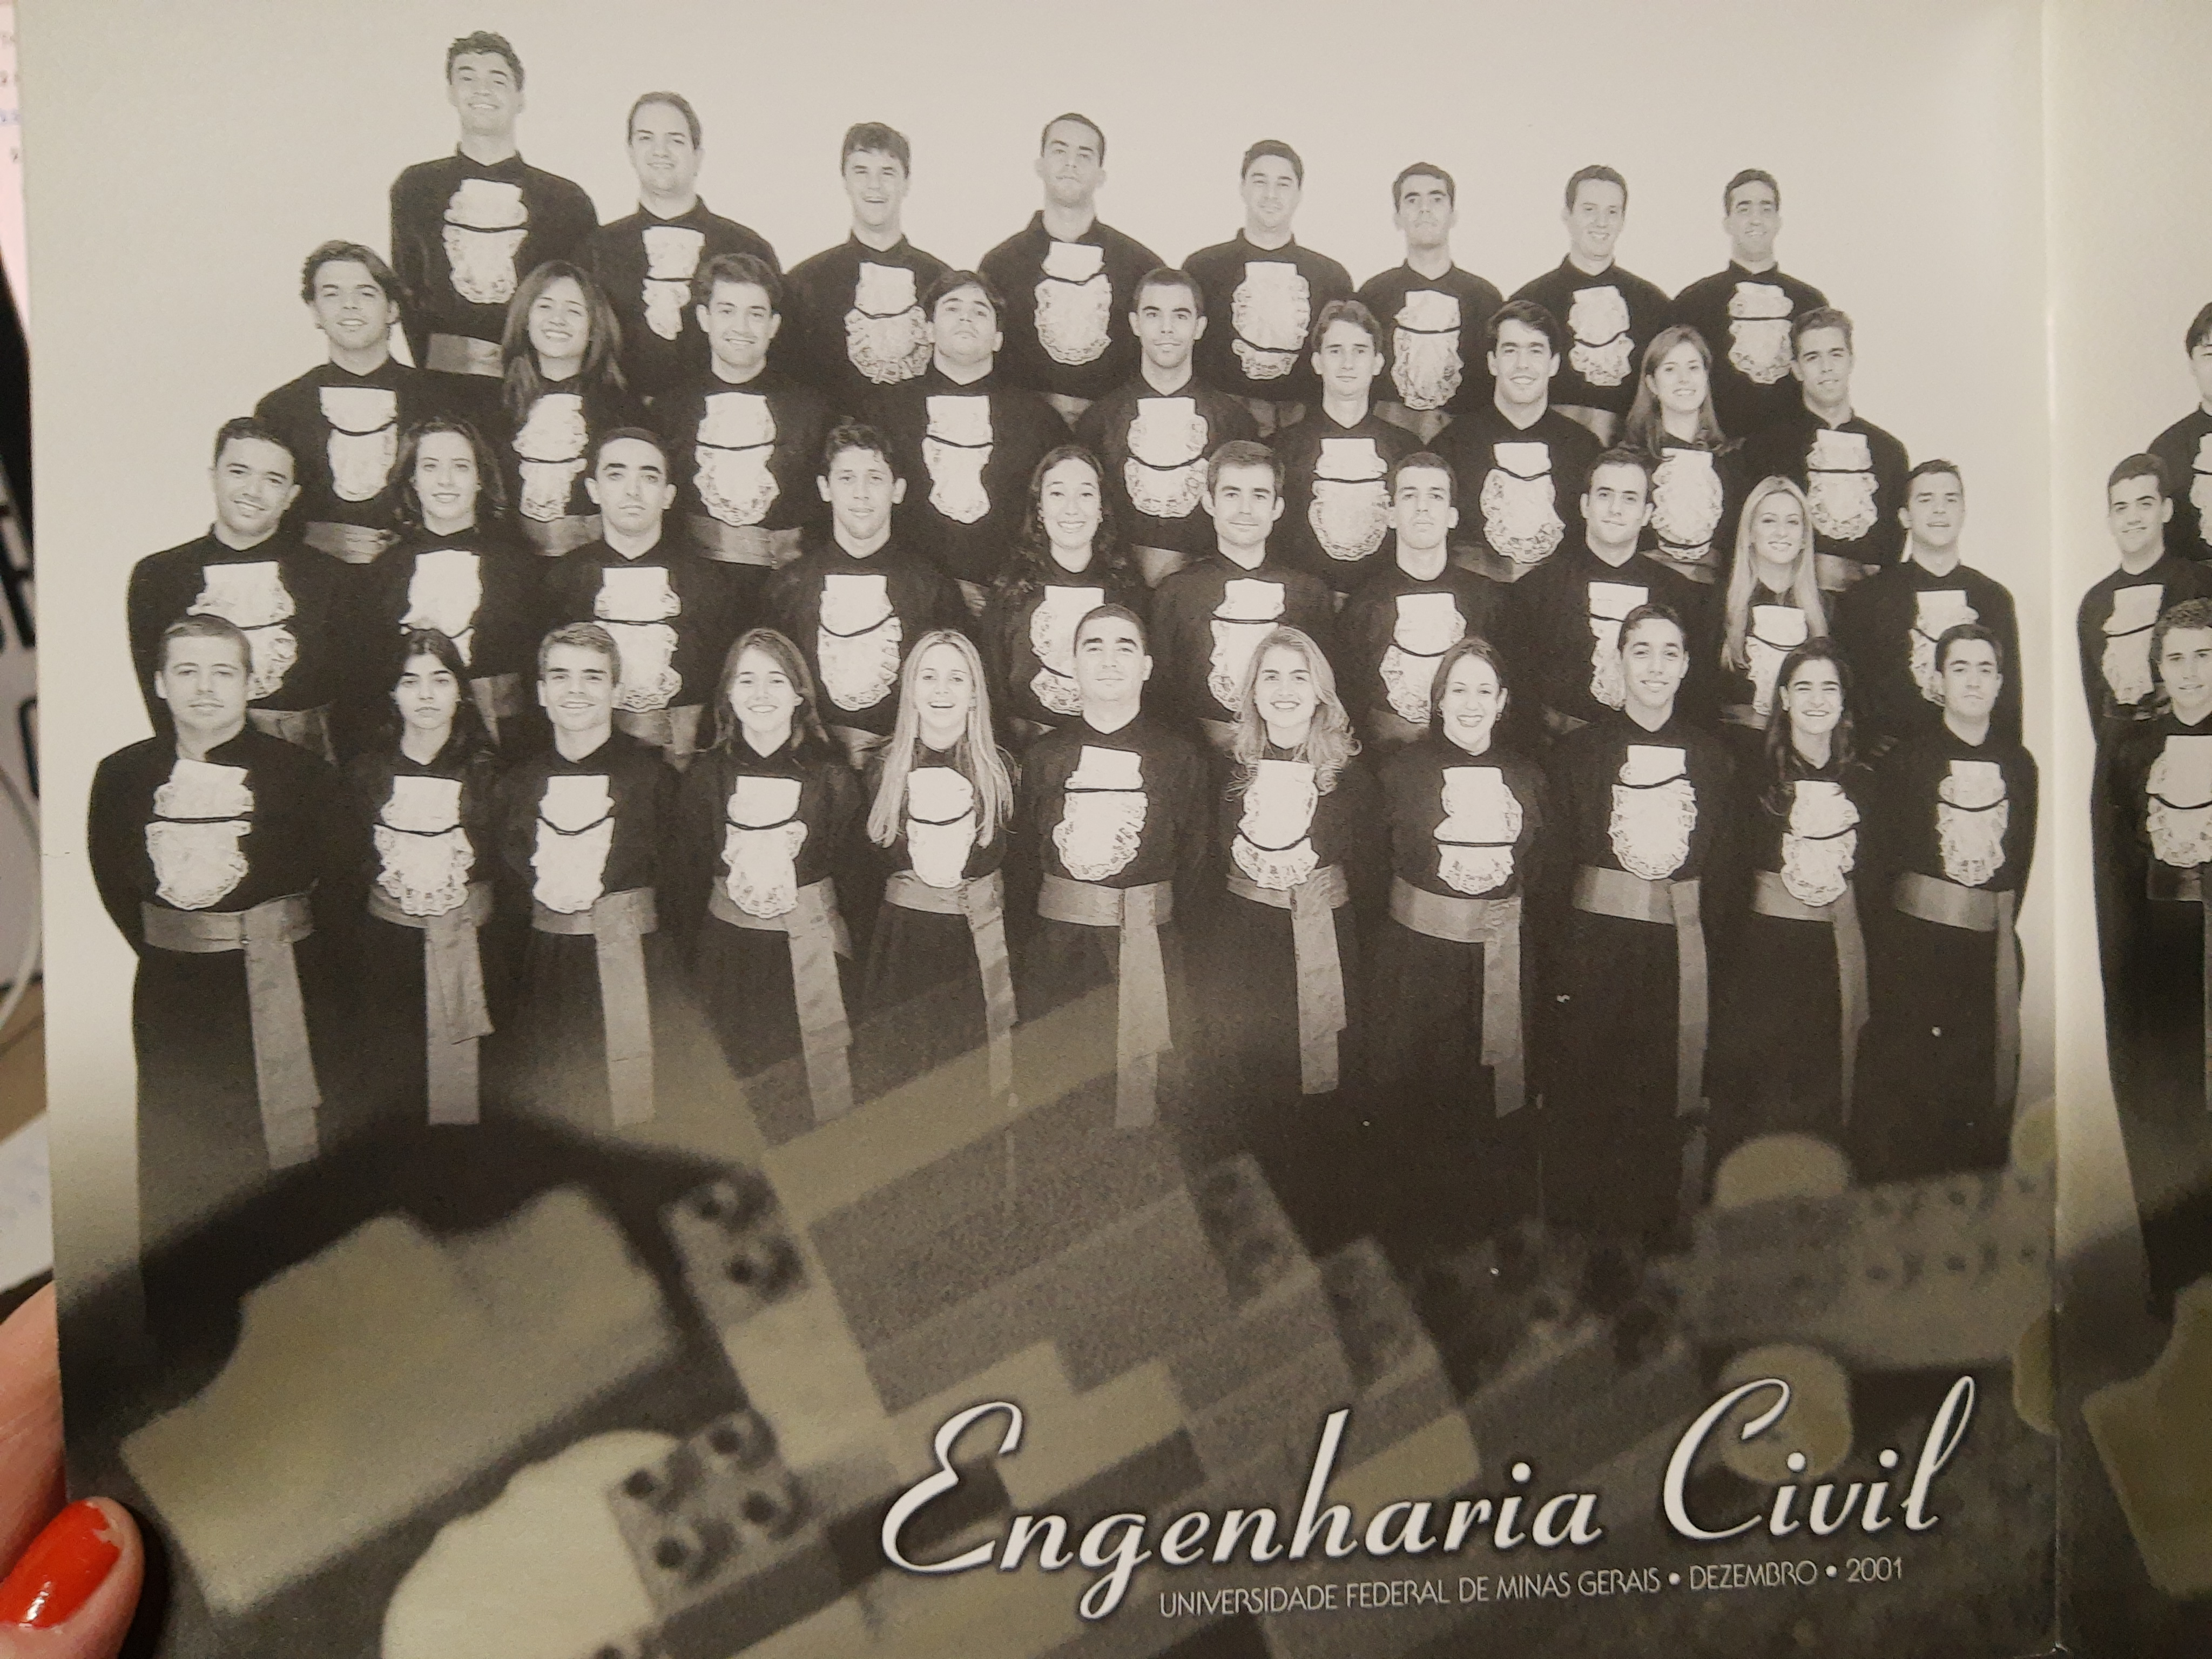
\includegraphics[width=1\linewidth]{img/forma} \caption{Formanda}\label{fig:forma}
\end{figure}

\hypertarget{puxf3s-graduauxe7uxe3o}{%
\section{Pós-Graduação}\label{puxf3s-graduauxe7uxe3o}}

Mestrado \#\#\# Especialização em Engenharia Ferroviária Especialização
em Engenharia Ferroviária Análise do Aumento de Confiabilidade das
Locomotivas da Rota do Grão a Partir da Implantação do Novo Quadro de
Tração da FCA

\hypertarget{mestrado-em-engenharia-de-transportes}{%
\subsection{Mestrado em Engenharia de
Transportes}\label{mestrado-em-engenharia-de-transportes}}

No mestrado, Modelo Neuro-Fuzzy para Escolha Modal no Transporte de
Cargas

\hypertarget{doutorado-em-geografia---tratamento-da-informauxe7uxe3o-espacial}{%
\subsection{Doutorado em Geografia - Tratamento da Informação
Espacial}\label{doutorado-em-geografia---tratamento-da-informauxe7uxe3o-espacial}}

A decisão de cursar o doutorado no programa de Geografia da PUCMinas
teve muito coração envolvido. Coração para decidir não buscar programas
fora de Belo Horizonte; coração apaixonado pela Geografia; coração
batendo fora do peito. Dizem por aí que ser mãe é ter o coração batendo
fora do peito. Concordo plenamente!

Decidi começar devagar e conhecer esse campo do conhecimento para
entender se havia possibilidade de incrementar minha formação em
transportes. Em 2010, com Sofia, minha primeira filha, com 3 meses, me
inscrevi na disciplina isolada ``Evolução do Pensamento Geográfico.''
Existem pessoas que quando passam por nossas vidas deixam marcas
indeléveis. Uma delas foi o professor \emph{Oswaldo Bueno Amorim Filho}.
Professor Oswaldo conseguiu, com sua capacidade de tecer o raciocínio e
coordenar a imensidão conceitual e temporal que são as múltiplas
geografias de maneira brilhante. Não tive como não me apaixonar pelas
infinitas possibilidades e caminhos epistemológicos, por vezes
ontológicos, de explorar fenômenos físicos e humanos. Ali nascia a
geógrafa que escreve esse memorial. Isso mesmo: GEÓGRAFA.

No semestre seguinte cursei \ldots.

No final de 2010 participei do processo seletivo do doutorado e
ingressei formalmente nesse mundo de novos horizontes e perspectivas. Na
escolha do orientador, me encaminharam para um professor bem .
Entretanto, optei por buscar um orientador que contribuísse para minha
formação como geógrafa, entendendo as implicações dos estudos
geográficos e seu desafios. Foi quando conversei com o professor
\emph{Alexandre Alves Magno Diniz}. Além de excelente profissional, cuja
área de especialização estava alinhada às minhas pretenções de trabalhar
com a geografia dos transportes, é uma pessoa humana, gentil e
disponível.

Demoramos um bom tempo entre o meu ingresso no programa e a definição da
pesquisa. Precisei fazer 48 créditos para poder cumprir o mínimo
requisito para a titulação como doutora. Parece muito, mas apesar dos
dois anos cursando disciplinas, eu queria até mais.

No início de 2013 meu marido (mais uma vez a ideia de \textbf{reduzir
distâncias} predomina nas minhas decisões pessoais, acadêmicas e
profissionais) conseguiu uma bolsa de seis meses na Université de Lyon
para desenvolver a parte experimental de sua pesquisa. Havia bolsas
disponíveis na PUCMinas para doutorado sanduíche e consegui também um
programa para que pudéssemos caminhar juntos nessa jornada. No final de
junho de 2013 desembarcamos, eu, Patrick, Sofia, João e minha mãe no
aeroporto Saint Exupéry. Muita apreensão, novidades e desapegos.
Atravessar o Atlântico com um bebê de seis meses e uma criança de 3 anos
já seria uma aventura. Atravessa o Atlântico com os pequenos para morar
por seis meses era uma enorme aventura com um pouco de loucura. Minha
mãe foi conosco para que fosse possível trabalharmos e, ao mesmo tempo,
prover cuidados ao João. Sem ela, essa aventura não teria sido possível!
Nos acomodamos em um hotel de maneira provisória até que encontrássemos
uma moradia para nossa estadia. Mais uma vez, a decisão passou por um
equilíbrio entre \textbf{distâncias} para que a localização do nosso lar
fosse o mais \textbf{central} possível em relação aos nossos
laboratórios e à vida cotidiana das crianças e de minha mãe.
Curiosamente Patrick precisava se deslocar para o extremo nordeste da
região de Lyon e eu para o extremo sudeste. Experiências fantásticas
foram apreendidas ao viver em uma cidade desconhecida, com desafios
locacionais e culturais, mas sem impedâncias para o deslocamento das
pessoas. Não precisamos de automóvel individual para exercer nenhuma das
funções cotidianas. As estações do metrô, o acesso aos ônibus
articulados, a confiabilidade nas tabelas de horários dos sistemas e até
mesmo a tarifa eram \textbf{acessíveis}. População em situação de
vulnerabilidade, famílias com muitos filhos e outros grupos específicos
contavam com subsídios públicos proporcionais às suas necessidades. Quem
pode mais, paga mais. Quem pode menos, paga menos.

Falar das férias, da forma de trabalhar da simplicidade do modo de vida,
do direito à cidade e dos desafios de viver longe.

ANÁLISE ESPACIAL DOS PREÇOS DE PRODUTOS ALIMENTÍCIOS NO VAREJO DE BELO
HORIZONTE E A SUA RELAÇÃO COM A RENDA MÉDIA DA POPULAÇÃO de muita
introspecção e reflexão.

\begin{figure}
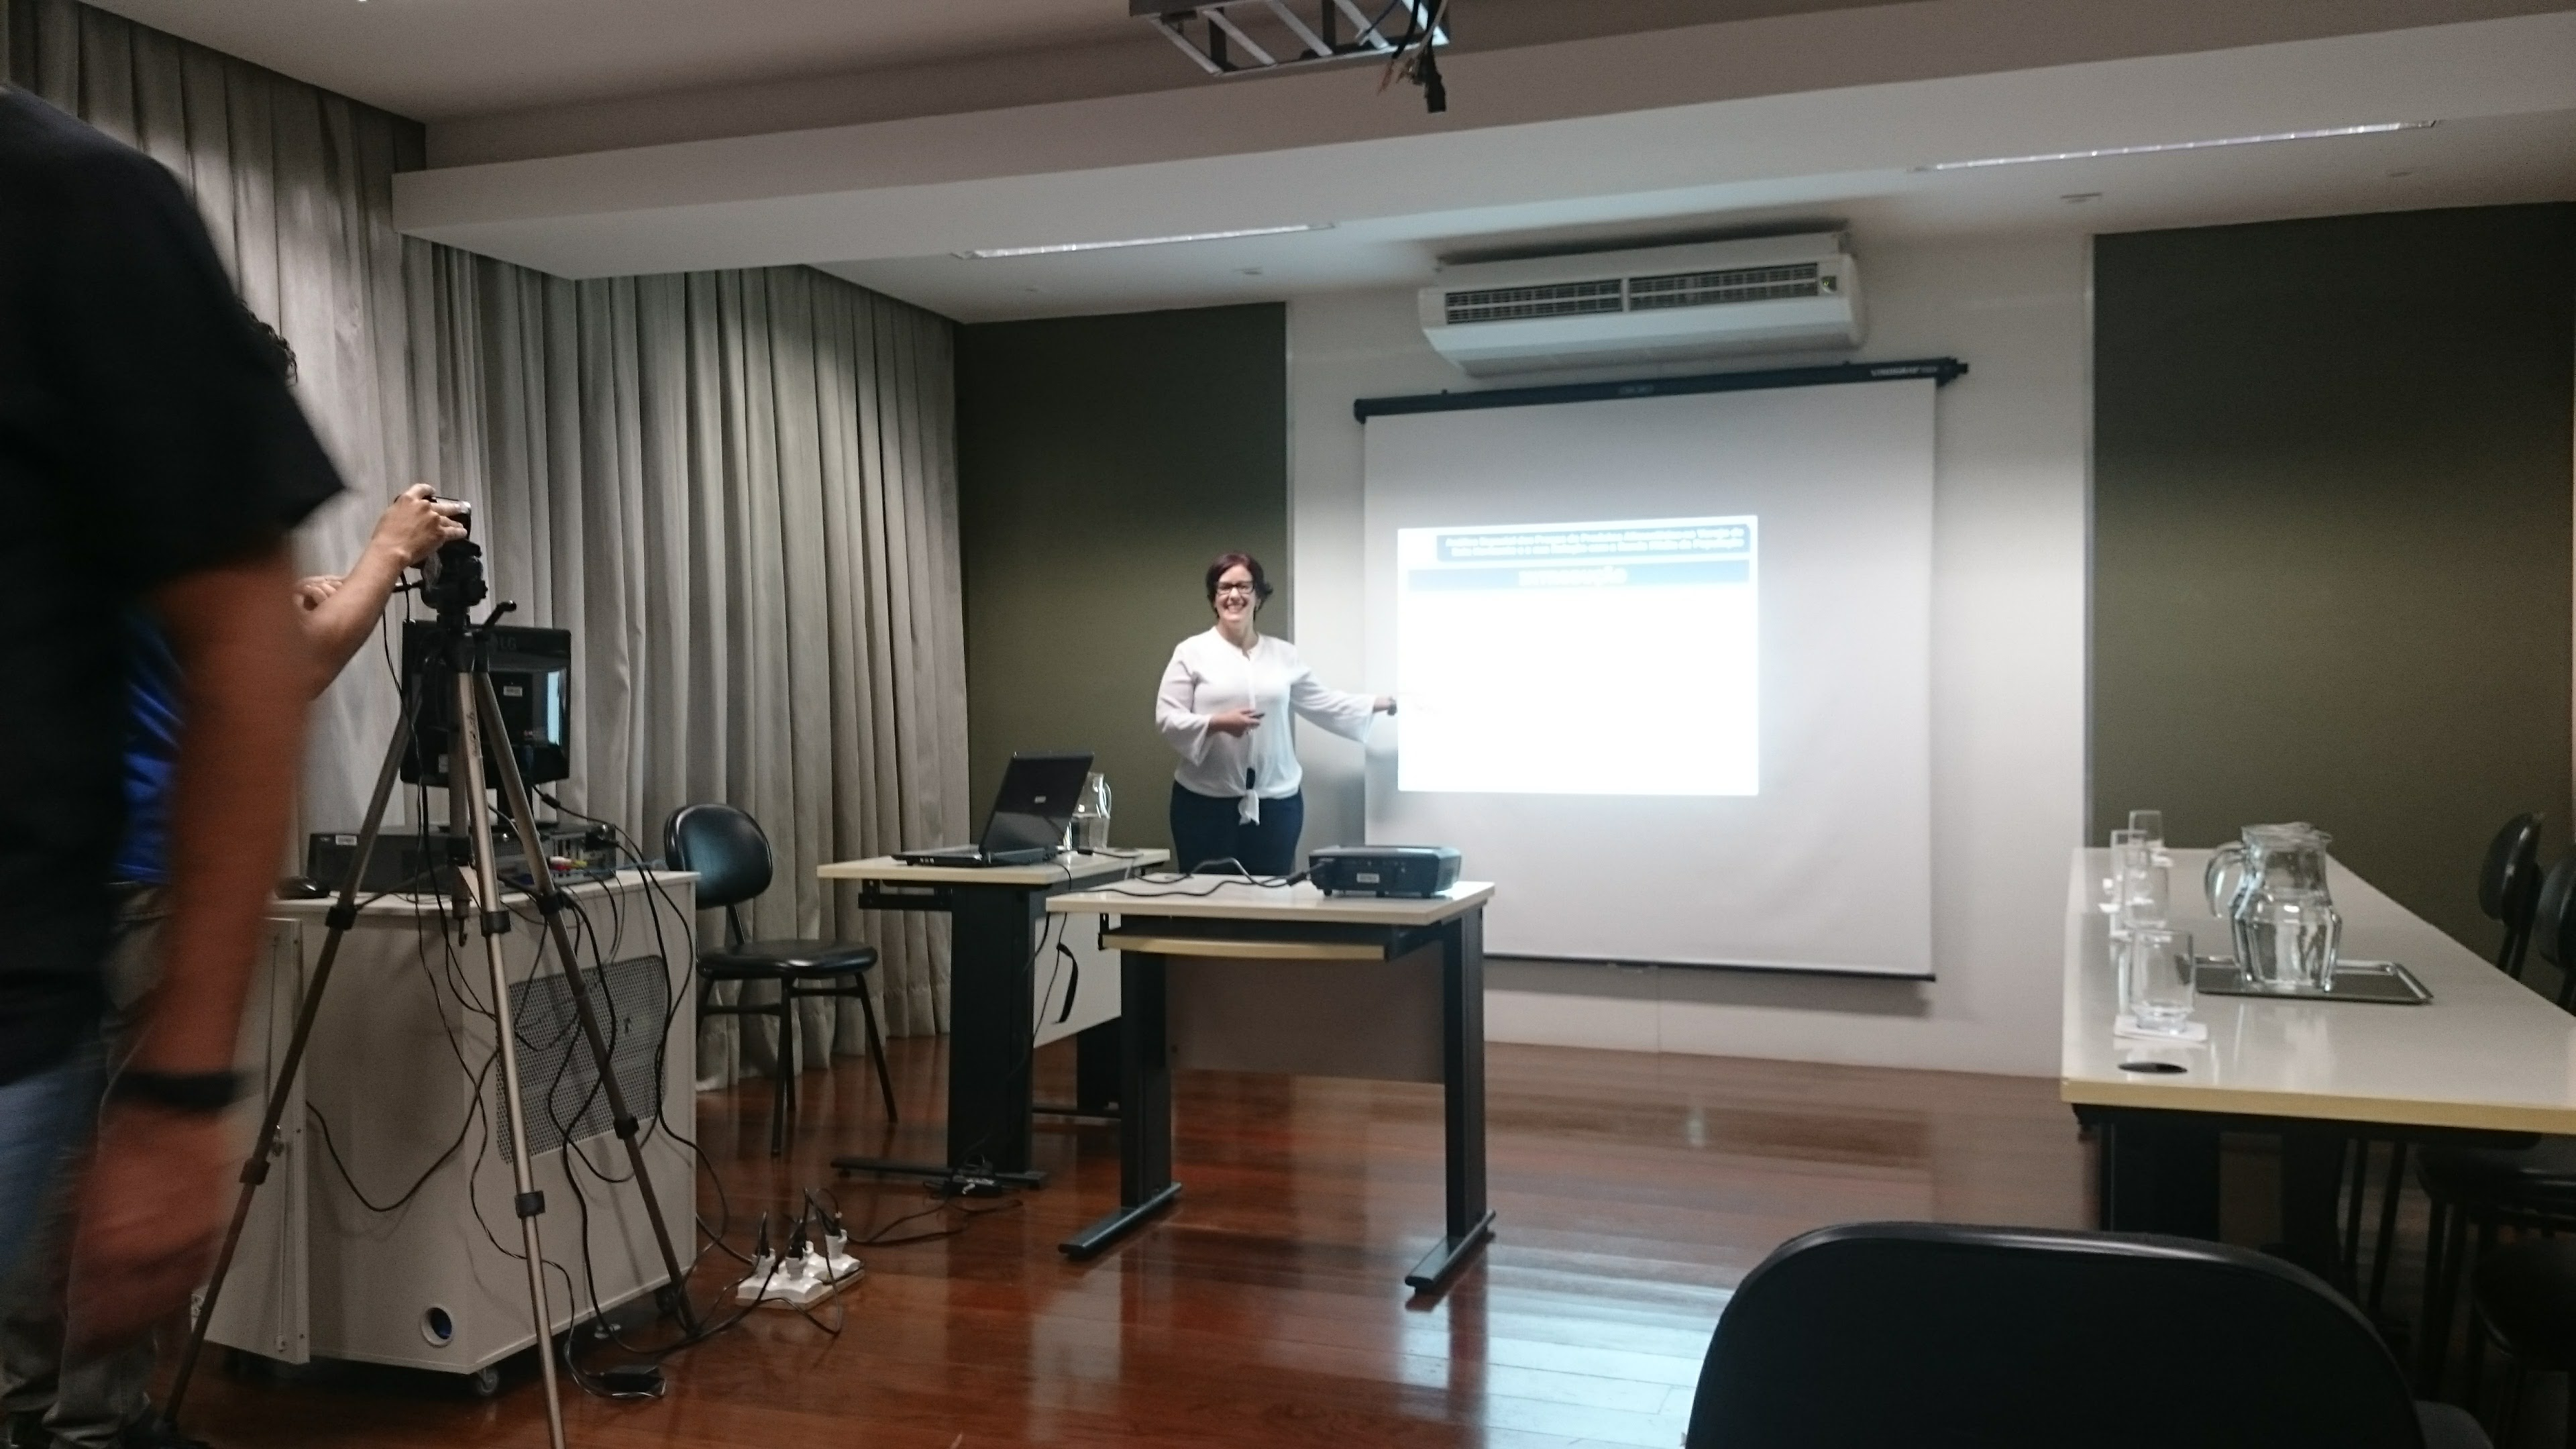
\includegraphics[width=1\linewidth]{img/defesa} \caption{Formanda}\label{fig:defesa}
\end{figure}

\hypertarget{atuauxe7uxe3o-como-docente}{%
\section{Atuação como docente}\label{atuauxe7uxe3o-como-docente}}

\hypertarget{cursos-tuxe9cnico-e-de-graduauxe7uxe3o}{%
\subsection{Cursos técnico e de
Graduação}\label{cursos-tuxe9cnico-e-de-graduauxe7uxe3o}}

\hypertarget{programas-de-puxf3s-graduauxe7uxe3o-stricto-sensu}{%
\subsection{Programas de Pós-Graduação Stricto
Sensu}\label{programas-de-puxf3s-graduauxe7uxe3o-stricto-sensu}}

No dia 19/05/2017 formalizei meu credenciamento no Programa de
Pós-graduação em Geotecnia e Transportes (PPGGT) da UFMG. O programa
precisava da participação de mais docentes e, caso eu quisesse progredir
na minha carreira de pesquisadora, precisaria desse espaço.

A primeira disciplina que lecionei foi \emph{Geografia dos Transportes}.
Foi um sonho. Uma energia maravilhosa da turma ao entender
condicionantes da engenharia que estão diretamente relacionadas à
localização das atividades, à estrutura morfológica das cidades e
regiões,

A atuação na UFMG é muito gratificante. Excelentes estudantes e
pesquisadores em formação e autonomia para desenvolvimento dos projetos
de pesquisa e dos trabalhos acadêmicos. Entretanto, a UFMG, apesar de
ter sido meu berço acadêmico, não é minha casa. É muito difícil
manter-me efetivamente colaborativa ao programa com a \textbf{distância}
institucional. Tentei algumas vezes coordenar os trabalhos de alunos
bolsistas de iniciação científica do CEFET-MG com alunos do mestrado
PPPGT, mas a \textbf{distância} física também era um limitador para essa
interação. Talvez, a partir das nossas experiência no contexto remoto,
poderemos viabilizar com mais assertividade a estruturação de uma rede
de suporte e a coordenação do desenvolvimento dos projetos de pesquisa.
Mais uma vez, a \textbf{distância} determina minhas escolhas. De forma
mais pragmática, atuar no PPGGT é um exercício de desapego, pois apesar
de UFMG e CEFET-MG serem duas instituições de ensino superior federais,
não há cessão dos docentes para atribuição dos encargos acadêmicos de
maneira colaborativa. Assim, para o CEFET-MG, essa atividade no PPGGT
torna-se um encargo adicional eletivo para o docente, não sendo
contabilizado nas apurações de atividades acadêmicas do docente
formalmente. Acredito que ainda tenhamos um longo caminho até que
possamos efetivamente entender que sem colaboração, não conseguimos
produzir conhecimento.

Em 31/07/2021 encerra-se meu credenciamento no PPGGT. É o fechamento de
um longo ciclo de idas e vindas na UFMG. Segue sendo meu berço
acadêmico, mas preciso caminhar e o CEFET-MG é uma instituição que
precisa do meu trabalho dedicado e que possibilita esse trabalho com uma
série de incentivos.

Paulo 1. Clarissa Pontes Melo. Análise da macroacessibilidade de
pedestres idosos sob a ótica da qualidade do espaço urbano. 2019.
Dissertação (Mestrado em Geotecnia e Transportes) - Universidade Federal
de Minas Gerais, . Orientador: Renata Lúcia Magalhães de Oliveira.

\begin{enumerate}
\def\labelenumi{\arabic{enumi}.}
\setcounter{enumi}{1}
\item
  André Augusto Cunha Libânio. AVALIAÇÃO DA ACESSIBILIDADE EM CIDADES
  BRASILEIRAS. 2018. Dissertação (Mestrado em Geotecnia e Transportes) -
  Universidade Federal de Minas Gerais, . Orientador: Renata Lúcia
  Magalhães de Oliveira.
\item
  Paulo Henrique Góes Pinto. Identificação e qualificação de
  centralidades urbanas por meio de estrutura morfológico-funcional: um
  estudo de caso para a RMBH. 2018. Dissertação (Mestrado em Geotecnia e
  Transportes) - Universidade Federal de Minas Gerais, . Orientador:
  Renata Lúcia Magalhães de Oliveira.
\item
  José Moreira Gonçalves. Atração de Viagens de Carga em Indústria
  Automobilística de Máquinas Agrícolas e Rodoviárias. 2017. Dissertação
  (Mestrado em Engenharia de Transportes) - Universidade Federal de
  Minas Gerais, . Orientador: Renata Lúcia Magalhães de Oliveira.
\item
  Gabriela Pereira Lopes. Uma Análise da Localização de Instalações
  Logísticas versus Geração de Viagens e os Impactos na mobilidade
  urbana em Belo Horizonte. 2016. Dissertação (Mestrado em Engenharia de
  Transportes) - Universidade Federal de Minas Gerais, . Coorientador:
  Renata Lúcia Magalhães de Oliveira.
\end{enumerate}

Em 2020 credenciei-me no Programa de Pós-Graduação em Administração do
CEFET-MG.

Tenho enormes dificuldades com caixinhas

\hypertarget{pruxeamios-e-homenagens}{%
\section{Prêmios e homenagens}\label{pruxeamios-e-homenagens}}

Funding and Prizes

Productivity research grant - CNPq

National Council for Scientific and Technological Research

Brasília, Brazil

2019 - 2022

Grant number: 312750/2018-8

One of the best Papers presented at PLURIS 2018

Publication in Revista Portuguesa de Estudos Regionais as a prize for
being among the 12 best papers presented in PLURIS 2018 (Congresso
Luso-Brasileiro para o Planejamento Urbano, Regional, Integrado e
Sustentável).

Lisbon, Portugal

2018

Como docente, recebi oito homenagens de alunos formandos dos cursos
técnico em Transportes e Trânsito e Engenharia de Produção Civil do
CEFET-MG, do curso de Administração da Fundação Comunitária de Ensino
Superior de Itabira - FUNCESI e do curso de Administração da Faculdade
Novos Horizontes.

\hypertarget{atividades-e-projetos-de-pesquisa}{%
\section{Atividades e Projetos de
Pesquisa}\label{atividades-e-projetos-de-pesquisa}}

Em 2017, em parceria com a profa. Leise Kelly da UFMG,

Comunicação e fomento à discussão por meio da organização do I Fórum de
Logística Urbana, em parceria com a UFMG e com a UFT.

Como pesquisadora, também tenho colaborado com diferentes periódicos,
nacionais e internacionais, como revisora ad hoc. Dentre eles, a revista
Transportes, IEEE Access, Sustainable Cities and Society, Research in
Transportation Economics, Transportation Research Record e Urban Rail
Transit. Hoje faço parte do corpo editorial das revistas Caderno de
geografia e da Revista Brasileira de Transportes.

Tenho participado de bancas de avaliação de trabalhos de conclusão de
Doutorado, Mestrado, Especialização e graduação. O escopo geográfico
dessa participação é bastante amplo, destacando o Programa de
Pós-Graduação em Modelagem Matemática e Computacional do CEFET-MG, o
curso de engenharia civil da UFT, o programa de pós-graduação em
Engenharia de Transportes da UFC, o curso de engenharia de produção da
UFSCar - Sorocaba,

Tenho investido bastante no processo de internacionalização das minhas
atividades como pesquisadora. Desde 2015 tenho participado de
conferências no exterior e de redes de pesquisa.

City Logistics NIUMAR Projetos de pesquisa Alguns dos projetos de
pesquisa que tenho trabalhado com preocupação:

o desenvolvimento de modelos de geração de viagens referentes às
instalações logísticas na Região Metropolitana de Belo Horizonte; local
de armazenagem em Belo Horizonte e na Região Metropolitana de São Paulo,
no que diz respeito aos aspectos morfológicos e funcionais da cidade; a
análise das mudanças temporais e espaciais relativas à distribuição das
instalações logísticas nas áreas metropolitanas; modelagem espacial do
transporte urbano de carga em cidades de médio porte e cidades
históricas; avaliação da localização potencial de uma rede de pontos de
coleta em Belo Horizonte; e planejamento orientado à acessibilidade para
promover a equidade considerando o acesso às funções urbanas e a
estrutura morfológica das cidades. Acabo de concluir uma pesquisa de
pós-doutorado com a Cátedra de Logística da Cidade e sob a orientação da
Professora Dra. Laetitia Dablanc. Minha função como pesquisadora de
pós-doutorado foi investigar as mudanças de localização dos armazéns em
diferentes áreas metropolitanas e sua relação com a estrutura urbana e
as práticas do mercado imobiliário.

\hypertarget{internacionalizauxe7uxe3o}{%
\section{Internacionalização}\label{internacionalizauxe7uxe3o}}

O processo de internacionalização também precisa de caminhos para que
seja possível instituir parcerias não só de pesquisa, mas também de
ensino. Nesse contexto, tenho participado das iniciativas institucionais
de formação dos docentes em English as a medium of instruction,
concluindo um capacitação de 40 horas em julho de 2020.

Em outubro de 2020 iniciei uma atividade de pesquisa em parceria com a
Logistics City Chair por meio de uma oportunidade de Pós-doutorado
remoto. O projeto foi intitulado e teve duração de 5 meses, estando em
fase de conclusão. Université Gustave Eiffel, UGE, França

Redução de desigualdades por meio do Planejamento da Acessibilidade e da
Mobilidade na Urbe Sustentável Soluções de logística urbana Análise
espacial aplicada a problemas urbanos

\hypertarget{atividades-e-projetos-de-extensuxe3o}{%
\section{Atividades e projetos de
Extensão}\label{atividades-e-projetos-de-extensuxe3o}}

Descrição: O Instituto de Atenção às Cidades - IAC, da UFT, por meio da
Fundação de Apoio Científico e Tecnológico do Tocantins ? FAPTO está
desenvolvendo o projeto ?Plano de Mobilidade Urbana Sustentável de
Paraíso do Tocantins?, proveniente de parceria firmada entre a UFT e a
Secretaria de Infraestrutura e Serviços Públicas da Prefeitura Municipal
de Paraíso do Tocantins. O objetivo desse plano é definir ações
estratégicas para se alcançar o cenário de mobilidade urbana desejado
para a cidade, em conformidade com a Política Nacional de Mobilidade
Urbana. A docente Renata Lúcia Magalhães de Oliveira foi convidada para
colaborar com esse projeto no desenvolvimento de estudos urbanos
orientados à acessibilidade para inclusão desse paradigma no diagnóstico
e propostas de intervenções. Posteriormente, tendo sido identificados os
indicadores de avaliação da acessibilidade urbana e do sistema de
mobilidade, a docente dará suporte técnico ao desenvolvimento de um
plano de monitoramento que ajude a identificar as mudanças provenientes
das intervenções propostas. A participação da docente faz-se necessária
frente à proposta de implementação do paradigma de planejamento
orientado à acessibilidade, na qual é especialista, como instrumento de
promoção de justiça social no planejamento da cidade visando a promoção
de acesso às oportunidades de maneira equitativa..

\hypertarget{eu-e-cefet}{%
\chapter{Eu e CEFET}\label{eu-e-cefet}}

No final de 2005 recebi um email da professora \emph{Heloísa Maria
Barbosa} do Departamento de Engenharia de Transportes e Geotecnia da
UFMG. Ela escreveu para me informar sobre um concurso que estava para
ser realizado no CEFET-MG, para a área de transportes. Eram duas vagas e
fiz inscrição despretenciosamente, pois a bibliografia para o concurso
era muito orientada à engenharia de tráfego. Decidi não me preparar para
o concurso, pois o prazo era exíguo e eu não conseguiria me organizar
para estudar. Apostei na ideia de que somos preparados ao longo da
formação acadêmica. E deu certo! Fiz a prova teórica, fiquei em segunda
colocação depois de escrever mais de 20 laudas. Entreguei a documentação
e sorteiei meu tema para a prova didática: Projetos Viários. Heloísa era
um dos membros da banca e tinha sido minha professora desse conteúdo
especificamente. Como eu poderia ministrar uma aula para minha
professora de um assunto que ela me ensinara e sobre o qual eu não tinha
me especializado?

Resolvi concentrar meus esforços na organização pedagógica da aula,
elaborando um plano de aula estruturado e destacando muito mais a
proposta do que o conteúdo. Naquele momento eu já tinha alguns anos de
experiência como professora, apesar de nenhuma qualificação formal
docente. Acho que a aula foi boa, pois fui aprovada para uma das vagas
e, no dia 10 de fevereiro de 2006, tomei posse.

Ingressei no CEFET-MG na coordenação de curso técnico em Transporte e
trânsito. Não éramos um departamento. Éramos duas coordenações de curso
que contemplavam o técnico em Transportes e Trânsito e o técnico em
Estradas cada uma. Tudo era novidade. Desde a ideia de lecionar para
adolescentes (eu me sentia e até hoje me sinto adolescente), até a
estrutura de uma Instituição de Ensino pública. Prontamente recebi o
cargo de coordenação de laboratórios dos cursos, o que me proporcionou
uma aprendizagem rápida sobre como funcionava a gestão institucional, os
processos de compras e pregões, a gestão da demanda por insumos
laboratoriais. Há alguns anos não via um aparelho de Casagrande
(confesso que precisei pesquisar o nome para escrevê-lo aqui!) e
precisei reaprender um pouco daquele universo da geotecnia e conhecer
implementações em asfaltos, infra e superestrutura viária. Por meio
dessa atuação como coordenadora de laboratório conheci muitas pessoas na
instituição. Conheci a estrutura organizacional. Naquela época ainda
havia pouca formalização dos processos institucionais e, portanto, as
relações pessoais eram essenciais para que os processos fossem
executados. Não havia digitalização dos meios de formalização das
demandas e dos posicionamentos institucionais e pouca alocação de
recursos humanos dedicados às funções administrativas. Nós,
coordenadores, éramos responsáveis por redigir atas, memorandos,
distribuir documentos fisicamente pelo campus. Confesso que essa
pessoalidade e a morosidade na condução dos processos administrativos me
incomodaram bastante, e tudo o que pude ``digitalizar'' dentro da
coordenação, o fiz.

Logo passei a ser coordenadora do curso de Estradas e em seguida de
Transportes e Trânsito. Estive à frente de pelo menos uma função de
coordenação até 2009, quando gozei licença maternidade. Dentre as
atividades administrativas que já exerci, a coordenação de cursos é a
mais interessante. Ela contempla a participação ativa em órgãos
colegiados responsáveis pelas discussões pedagógicas e curriculares.
Aprendi muito sobre como funcionam as referências curriculares nacionais
para o ensino profissional e tecnológico e como são base para a
construção da estrutura dos cursos técnicos. Discuti institucionalmente
e construi argumentações para o MEC com foco na necessidade de adequação
do curso técnico em Transportes e Trânsito ao Catálogo Nacional de
Cursos Técnicos (e vice-versa). Fiz inúmeras reuniões com estudantes e
familiares na busca de soluções para as dificuldades das famílias e dos
estudantes em relação à instituição.

Como docente, entre 2006 e 2016\footnote{Houve períodos de licença
  maternidade em 2009 e 2012 e o período de licença para capacitação
  entre 2011 e 2014 nesse período.}, lecionei essencialmente nos cursos
técnicos da coordenação que tornou-se Departamento de Engenharia de
\textbf{Transportes} quando da implementação do curso de Engenharia de
\textbf{Transportes}. Ministrei, de maneira consistente, as disciplinas
``Gerenciamento de Transportes de Carga,'' ``Operação de Transportes de
Cargas,'' ``Políticas e Planejamento de Transportes'' e
``Administração'' para os cursos técnicos.

Em 2008 elaboramos e implementamos a reestruturação dos cursos técnicos
integrados, e as disciplinas tornaram-se anuais, com alteração da
estrutura curricular dos cursos. As disciplinas dos cursos técnicos na
modalidade concomitância externa e subsequente (quando o estudante não
cursa o ensino médio de maneira integrada ao ensino profissionalizante)
eram ofertadas no turno noturno e a estrutura curricular não sofreu
alterações importantes. Entretanto, para os cursos intergados diurnos
(ensino médio profissionalizante), as disciplinas que passei a ministrar
foram denominadas ``Logística,'' ``Transporte de Cargas Eventualmente
ministrei algumas disciplinas para a Engenharia de Produção Civil,
como''Distribuição Física de Produtos e Layout" e ``Logística.''

Em novembro de 2009 deixei as funções de coordenação de
cursos/laboratórios para ser mãe. Imersa na licença maternidade, me
ausentei de todas as atividades profissionais e acadêmicas. Naquele ano,
antes da licença, participei da comissão de reestruturação do projeto
político-pedagógico do curso de Engenharia de Transportes, que foi
aprovado institucionalmente em 2012 (@ref(fig:eng)). Era um projeto
muito especial, especialmente por se tratar de mais uma oferta de cursos
de engenharia gratuitos noturnos, se consolidando como uma síntese dessa
área de conhecimento na formação de profissionais e num processo de
inclusão devido ao acesso a estudantes que precisam trabalhar.

\begin{figure}
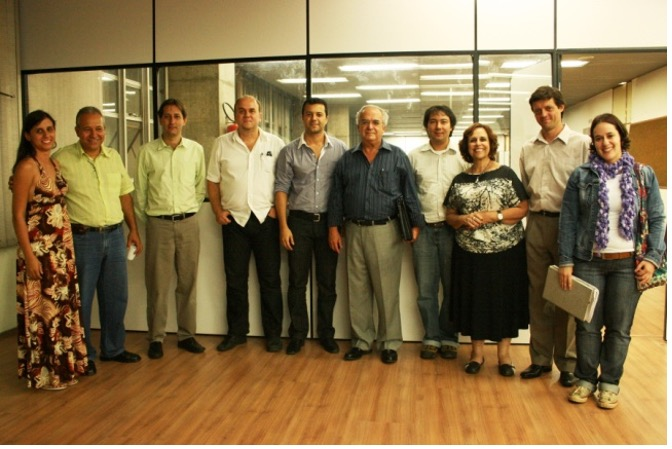
\includegraphics[width=1.3\linewidth]{img/Imagem1} \caption{Engenharia}\label{fig:eng}
\end{figure}

Retornando da licença em 2010, já estava cursando disciplinas isoladas
no programa de geografia da PucMinas e conciliei as atividades
acadêmicas e administrativas até que, em 2011, gozei de licença para
capacitação. Além de todo investimento público na minha formação
acadêmica a partir do ensino superior, o CEFET\_MG foi muito importante
na continuidade da minha formação. A instituição efetivamente investe na
qualificação do capital humano. Obtive licença de 3,5 anos e fomento
financeiro para pagamento das mensalidades do doutorado.

Como os assuntos do coração permeiam toda minha vida profissional e
acadêmica\footnote{E eu adoro uma aventura: coordenar o doutorado com
  mais um filhote a caminho. Confesso que os filhotes são maravilhosos,
  mas a limitação cognitiva hormonal durante a gravidez e o puerpério
  são um pouco restritivas!}, engravidei do João em 2012, ainda cursando
disciplinas do doutorado. João nasceu em dezembro daquele ano e, seis
meses depois, embarcávamos para um período de doutorado-sanduíche na
França. Não fiquei imersa na maternidade durante a licença após o
nascimento do João, pois vivia novos desafios acadêmicos\footnote{Toda
  mãe merece um segundo filho; tudo é mais leve e gostoso. Aprendemos
  que bebês são uma fortaleza e os seres mais adaptáveis e resilientes
  do mundo.}.

Em 2015, apesar de ainda estar em fase de conclusão da minha tese de
doutorado, retornei às atividades no CEFET-MG. Assumi a sub-coordenação
da Engenharia de Transportes já com um arranjo para que eu me tornasse
coordenadora assim que o doutorado fosse concluído; e assim foi feito.

Em 20 de agosto de 2015 defendi o doutorado e assumir a coordenação de
Engenharia de Transportes. 2015 e 2016 foram anos de muito trabalho,
pois o curso estava em implementação. Como coordenadora, além das
atribuições da rotina normatização do colegiado, fui responsável:

\begin{itemize}
\item
  pela revisão de pré e correquisitos da matriz curricular do curso, em
  alinhamento com a equalização de disciplinas da instituição;
\item
  pela regulamentação do colegiado do curso de graduação em Engenharia
  de Transportes;
\item
  pela instituição de critérios para classificação de candidatos a vagas
  remanescentes para obtenção de novo título;
\item
  pela regulamentação do núcleo docente estruturante do curso de
  graduação em Engenharia de Transportes;
\item
  pelas atividades de acompanhamento de estágios curriculares do curso
  de graduação em Engenharia de Transportes;
\item
  - pela coordenação do início das discussões sobre um currículo mínimo
  e as habilitações profissionais entre os cursos de Engenharia de
  transportes e mobilidade do país. O CEFET-MG sediou a primeira reunião
  dos representantes dos cursos.
\end{itemize}

Participei ainda da construção do regulamento para os trabalhos de
conclusão de curso para o curso de graduação em Engenharia de
Transportes e de todo o processo de organização para recebermos o MEC em
sua visita de reconhecimento do curso. Após a visita no final de 2019, o
curso recebeu nota máxima em seu reconhecimento!

De 2017 a 2019, além daquelas ministradas nos cursos técnicos, lecionei
as seguintes disciplinas para o curso de engenharia de transportes:

\begin{itemize}
\item
  Introdução à engenharia de transportes;
\item
  Tópicos especiais: Geografia dos Transportes;
\item
  Logística Urbana;
\item
  Orientação de estágio supervisionado;
\item
  Trabalho de conclusão de curso I;
\item
  Trabalho de conclusão de curso II;
\item
  Gestão do transporte de cargas;
\item
  Planejamento ferroviário.
\end{itemize}

Ministrar a disciplina ``Introdução à Engenharia de Transportes'' foi
muito especial. Primeiro, por ser a disciplina responsável por
apresentar essa área de conhecimento de forma integrada para os
estudantes. Segundo, porque o doutorado em Geografia me fez entender a
necessidade do contexto social, econômico, político, ambiental,
cultural, histórico e locacional para que possamos entender quaisquer
processos naturais ou sociais. Assim, para essa disciplina, precisei:

\begin{itemize}
\item
  fazer uma discussão dos caminhos da humanidade nas construções
  tecnológicas (\protect\hyperlink{ref-harari2015a}{Harari 2015};
  \protect\hyperlink{ref-bazzo2013}{Bazzo and Pereira, Luiz 2013});
\item
  explorar a história da engenharia e os contextos para que essa área de
  conhecimento começasse a ser construída
  (\protect\hyperlink{ref-svinicki2013}{Svinicki and McKeachie 2013};
  \protect\hyperlink{ref-ensinod2006}{Schnaid et al. 2006};
  \protect\hyperlink{ref-uxealmorfilho2019}{Êlmor Filho 2019};
  \protect\hyperlink{ref-bazzo2013}{Bazzo and Pereira, Luiz 2013});
\item
  discutir com os estudantes fundamentos geográficos como a interação
  espacial em diferentes escalas e formas, impulsionou os adventos
  tecnológicos na construção histórica e geográfica dos sistemas de
  transportes (\protect\hyperlink{ref-modernt1992}{Hoyle, Knowles, and
  Institute of British Geographers 1992};
  \protect\hyperlink{ref-blunden1971}{Blunden 1971};
  \protect\hyperlink{ref-taaffe1973}{Taaffe and Gauthier 1973};
  \protect\hyperlink{ref-bavoux2005}{Bavoux 2005};
  \protect\hyperlink{ref-thegeog2004}{Hanson and Giuliano 2004};
  \protect\hyperlink{ref-shallat2010}{Shallat et al. 2010});
\item
  discutir os fundamentos tecnológicos das tecnologias de transporte.
\end{itemize}

Em 2020, comecei uma jornada renovadora no CEFET-MG. Mudei de
departamento e fui

No DCSA

Em funções administrativas institucionais, já participei e participo de
diferentes comissões temporárias e permanentes, como:

\begin{itemize}
\item
  Comitê de Ética em Pesquisa CEP/CEFET-MG;
\item
  Câmaras Temáticas da Comissão de Iniciação;
\item
  Participacão em Bancas Examinadoras do Concurso Público de Provas e
  Títulos para provimento de cargas da carreira de Magistério do Ensino
  Básico, Técnico e Tecnológico;
\item
  Participação em bancas examinadoras de processo seletivo simplificado
  para professores substitutos/temporários;
\item
  Outras comissões temporárias.
\end{itemize}

No meu primeiro semestre no DCSA, precisei lecionar a disciplina Gestão
da Qualidade. Havia 15 anos que não lecionava esse conteúdo e muito
havia mudado na minha maneira de ver o mundo organizacional, social e o
papel da docência nesse contexto. Confesso que Gestão da Qualidade não
seria minha, de longe, minha primeira opção. Vasculhei a documento das
vezes em que ministrei essa disciplina e verifiquei que não conseguiria
aproveitar nada do que havia produzido anteriormente.

Penso que podemos ministrar qualquer conteúdo sob diferentes
perspectivas. Em 2005, quando lecionei Gestão da Qualidade, tive uma
abordagem positivista da disciplina, apresentando ferramentas e
funcionalidades para os estudantes. É usualmente a proposta dos
livros-texto. Entretanto, em 2020, meu esforço ao ministrar essa
disciplina foi fazer uma análise crítica da Gestão da Qualidade
considerando:

\begin{itemize}
\item
  a cronologia dos conceitos e como foram incrementalmente sendo
  alterados;
\item
  a função organizacional privada e os desafios contemporâneos relativos
  à responsabilidade social e ambiental;
\item
  o repensar do papel da padronização de processos em um contexto de 4a
  revolução industrial em que máquinas são responsáveis por processos
  decisórios e as competências mais demandas dos profissionais são a
  criatividade, a capacidade de colaboração, a empatia, a flexibilidade,
  a capacidade de comunicação, o pensamento crítico, a liderança, a
  iniciativa de antever situações que podem ser inadequadas ao processo
  de produção.
\end{itemize}

Foi muito interessante explorar discussões mais conceituais sobre os
processos de produção do que apenas instrumentalizar os estudantes.

Hoje faço parte do colegiado do Programa de Pós-Graduação em
Administração e da graduação em Administração.

\hypertarget{assuntos-do-corauxe7uxe3o}{%
\chapter{Assuntos do coração}\label{assuntos-do-corauxe7uxe3o}}

Essa seção merece um documento exclusivo. É a seção mais deliciosa deste
memorial! Apesar de toda sua importância, vou apenas fazer uma linha do
tempo com algumas fotos para aquecer o coração!

20/05/2001 - Primeiro dia juntos! 30/05/2001 - Começamos a namorar!

Namoro, Casamento, filhos\ldots{}

Namoro Morar junto e vida de gente grande

\hypertarget{para-onde-quero-ir}{%
\chapter{Para onde quero ir\ldots{}}\label{para-onde-quero-ir}}

A materinidade vem carregada de demandas, desafios e incertezas. Nossa
vida muda tanto que não conseguimos nos lembrar como éramos antes e o
que fazíamos com o tempo que nos sobrava. Seria intuitivo pensar que
mães são menos produtivas ou que o mundo do trabalho pode ser menos
importante após o nascimento dos filhos. Discordo desse pensamento que,
por vezes, domina nossa sociedade e acaba norteando algumas políticas
públicas e corporativas.

Quando minha primeira filha nasceu, nasceu uma nova Renata. Uma Renata
mais atenta ao mundo e mais responsável com seu entorno. Nasceu a Renata
que queria mudar o mundo! Sei que esse memorial é profissional, mas não
consigo dissociar os papéis sociais que exerço da minha emoção e dos
meus sentimentos.

A Renata-mãe, aos 30 anos, acreditava que conseguiria mudar o mundo.
Tornou-se mais rebelde às instituições, mais crítica e produtiva. Foi um
momento da minha vida muito significativo na transformação permanente
que vivermos.

Jane Jacobs, Jan Gehl e Lefebre.

\hypertarget{docuxeancia}{%
\section{Docência}\label{docuxeancia}}

Hoje penso que temos inúmeras perspectivas para explorar o mundo, os
fenômenos naturais, sociais e suas interações. Há algum tempo, tenho
entendido a minha responsabilidade como docente de me posicionar como
aquele ator no processo educacional que conduz o estudante à reflexão.
Sinto-me como uma curadora de instrumentos que promovam o pensamento
crítico de forma coordenada e incremental.

Edgar Morin Complexidade

Educação transdisciplinar e integral

Difusão de conhecimento e transferência tecnológica

A vida é cheia de mudanças e escolhas. Cada escolha que fazemos impacta
quem está no nosso \textbf{entorno} e aqueles que encontram-se muito
\textbf{distantes} de nós. Chegar à minha quarta década de vida tem sido
um experiência diferente daquelas vividas anteriormente. Aos 30,
pensamos muito mais no resultado material e imediato do trabalho que
desenvolvemos do que no singelo incremento potencial que cada nova
investigação pode trazer. Aos 30, pensamos que podemos mudar o mundo.
Aos 40, já temos certeza que não mudaremos o mundo, mas que podemos
trabalhar para promover o questionamento, a reflexão e a discussão, para
eliminar a dicotomia das argumentações, e para que, aos poucos, possamos
ver mudanças nas pequenas escolhas cotidianas que fazemos e que as
pessoas \textbf{próximas} fazem. Entendo que \textbf{próximos} são
aqueles que dividem o coração conosco, mesmo que \textbf{distantes} em
termos geográficos.

Extensão PET Recentemente fui convidada para assumir a função de
co-tutora do Programa de Educação Tutorial da Administração (PET-adm). É
uma equipe muito engajada e responsável. Os alunos são muito autônomos e
os projetos devem contemplar os eixos ensino, pesquisa e extensão.
Apesar da minha recente transição de docente para docente-pesquisadora,
penso que a extensão tenha uma importância muito grande no contexto
brasileiro.

Em trocas recentes com laboratórios internacionais, percebi que não
existe distinção entre atividades de pesquisa e extensão como há no
Brasil. Pelo contrário, a difusão do conhecimento e a transferência
tecnológica, em alguma dimensão, fazem parte da pesquisa científica.

Outro aspecto que tem me chamado a atenção após meu ingresso no
Departamento de Ciências Sociais Aplicadas e no Programa de
Pós-Graduação em Administração no CEFET-MG, tem sido a distinção
epistemológica entre pesquisa na Administração. Nossa área de
concentração é denominada Existe uma linha positivista e funcionalista,
que entende os processos de gestão

A difusão de conhecimento deve começar entre os pares. Tanto no programa
da UFMG como no do CEFET, sinto que não há um entendimento coletivo do
que cada pesquisador ou grupo desenvolve em seu trabalho acadêmico. O
mais comum é não dividirmos sala de aula e não consolidarmos parceria de
pesquisa entre os pares. Quero promover seminários acadêmicos que
permitam a troca de ideias, experiências, êxitos e frustrações no
desenvolvimento da pesquisa. Inicialmente, esses seminários seriam
internos, mas com o tempo, podemos espandir para a comunidade do
CEFET-MG e, a posteriori, abrir para o público em geral.

Entretanto, essa difusão, por mais interessante que seja, ainda tem a
limitação da linguagem e da abordagem. Não é palatável o suficiente para
\textbf{reduzir as distâncias} entre o entendimento coletivo e
individual de pessoas fora daquele campo de conhecimento e dos
especialistas. Vejo um enorme potencial no PET-Adm para o
desenvolvimento e implementações que consigam difundir o conhecimento de
maneira mais universal e efetivamente promover a transferência
tecnológica.

\hypertarget{refs}{}
\begin{CSLReferences}{1}{0}
\leavevmode\hypertarget{ref-bavoux2005}{}%
Bavoux, Jean-Jacques. 2005. \emph{Géographie des transports}. Paris:
Colin.

\leavevmode\hypertarget{ref-bazzo2013}{}%
Bazzo, Walter, and Pereira, Luiz. 2013. \emph{Introdução à Engenharia:
Conceitos, Ferramentas e Comportamentos}. 4a ed. Editora UFSC.

\leavevmode\hypertarget{ref-blunden1971}{}%
Blunden, W. R. 1971. \emph{The Land-Use/Transport System}. Pergamon.

\leavevmode\hypertarget{ref-uxealmorfilho2019}{}%
Êlmor Filho, Gabriel. 2019. \emph{Uma Nova Sala de Aula é Possível:
Aprendizagem Ativa Na Educação Em Engenharia}. LTC.

\leavevmode\hypertarget{ref-thegeog2004}{}%
Hanson, Susan, and Genevieve Giuliano, eds. 2004. \emph{The Geography of
Urban Transportation}. 3rd ed. New York: The Guilford Press.

\leavevmode\hypertarget{ref-harari2015a}{}%
Harari, Yuval N. 2015. \emph{Sapiens: a brief history of humankind}.
First U.S. edition. New York: Harper.

\leavevmode\hypertarget{ref-modernt1992}{}%
Hoyle, B. S., R. D. Knowles, and Institute of British Geographers, eds.
1992. \emph{Modern Transport Geography}. London ; New York: Belhaven
Press.

\leavevmode\hypertarget{ref-ensinod2006}{}%
Schnaid, Fernando, Milton Antônio Zaro, Maria Isabel Timm, and Ana Maria
Rosa, eds. 2006. \emph{Ensino de Engenharia: Do Positivismo à Construção
Das Mudanças Para o século XXI}. 1a ed. Porto Alegre, RS: UFRGS Editora.

\leavevmode\hypertarget{ref-shallat2010}{}%
Shallat, Todd, David Eberle, Larry Burke, Boise State University, and
College of Social Sciences and Public Affairs. 2010. \emph{Making
Livable Places: Transportation, Preservation and the Limits of Growth}.
Boise, Idaho: Boise State University, College of Social Sciences; Public
Affairs.

\leavevmode\hypertarget{ref-svinicki2013}{}%
Svinicki, Marilla D, and Wilbert J McKeachie. 2013. \emph{Dicas de
ensino: estratégias, pesquisa e teoria para professores universitários}.
\url{https://elibro.net/ereader/elibrodemo/126394}.

\leavevmode\hypertarget{ref-taaffe1973}{}%
Taaffe, Edward J., and Howard L. Gauthier. 1973. \emph{Geography of
Transportation}. Prentice-Hall Foundations of Economic Geography Series.
Englewood Cliffs, N.J: Prentice-Hall.

\end{CSLReferences}

\backmatter
\end{document}
